%\begin{comment}
\documentclass[11pt]{article}  % , titlepage
\usepackage{Common/toshi}
\begin{document}
%\end{comment}




%%%%%%%%%%%%%%%%%% section 3 %%%%%%%%%%%%%%%%%%%%%%%%%%%%%%%%%
\section{Line defects as transfer matrices}
\label{sec:line_defects}




%FIGURE
\begin{figure}
  \centering
    %\subfloat[\label{}]{  }
    %\subfloat[\label{}]{  }
    \begin{tikzpicture}[scale=1, font=\small, baseline=(x.base)]  \node (x) at (0,0) {\vphantom{x}};
      \def\pos{1cm}

        \node[align=center] (Q) at (0,0) {Quiver gauge theory \\ (class-$\CS$)};
        \node[above=1.6\pos of Q] (B) {Brane tiling};
        \node[right=2*\pos of Q] (Toda) {Toda CFT}; \node[right=0.8*\pos of Q] {$\simeq$};
        \node[above=1.6*\pos of Toda] (M) {M-theory setup};
        \node[left=2*\pos of Q, align=center] (I) {Integrable \\ lattice model};
        \node[above=1.6*\pos of I] (CS) {4d Chern-Simons};
        \node[below=1.2*\pos of Q, align=center] (T) {Transfer matrix/Wilson-'t Hooft line/Verlinde operator \\ acting on a quantum Hilbert space};
        %\node[below=1.6*\pos of Q, text opacity=0] (Tp) {(4) Transfer matrix/surface defect acting};

        \draw[semithick, arrows=-to] (B) to (Q);
        \draw[semithick, dashed, arrows=-to] (B.south west) to (I.north east);% node[above left,pos=0.5,align=center,font=\scriptsize] {general \\ prescription} (I.north east);
        \draw[semithick, color=red!50!black, arrows=-to] (B.east) to (M.west);
        \draw[semithick, color=red!50!black, arrows=-to] (B.west) to node[above,pos=0.5] {(4)} (CS.east);
        \draw[semithick, arrows=-to] (CS) to (I);
        \draw[semithick, arrows=-to] (M) to (Toda);
        \draw[semithick, arrows=-to] (M.south west) to node[below right=0.2cm,pos=0.5] {AGT} (Q.north east);

        \draw[thick, color=blue!50!black, arrows=-to] (T.north west) to[bend left=15] node[pos=0.5,left] {(1)} (I.south);
        \draw[thick, color=blue!50!black, arrows=-to] (T) to node[pos=0.5,right] {(2)} (Q);
        \draw[thick, color=blue!50!black, arrows=-to] (T.north east) to[bend right=12] node[pos=0.5,right] {(3)} (Toda.south);

    \end{tikzpicture}
    \caption{Structure of section \ref{sec:line_defects}. (1)}
    \label{fig:structure_line}
  \end{figure}






\subsection{Integrable lattice models of elliptic and trigonometric type}
\label{sec:QIS}

In this section we discuss the integrable system side of the
correspondence.  After reviewing L-operators, transfer matrices and
their relation to quantum integrable systems, we introduce an
L-operator for the elliptic dynamical R-matrix.  Then we define
fundamental trigonometric L-operators as certain limits of the
elliptic L-operator.  These fundamental L-operators are building
blocks of transfer matrices that correspond to Wilson--'t Hooft lines
in $\CN = 2$ supersymmetric circular quiver theories.


\subsubsection{L-operator and quantum integrable system}

Let $\hf$ be a finite-dimensional commutative complex Lie algebra and
$V$ a finite-dimensional diagonalizable $\hf$-module.  Choosing a
basis $\{v_i\}$ of $V$ that is homogeneous with respect to weight
decomposition, we denote the weight of $v_i$ by $h_i$ and the
$(i,j)$th entry of a matrix $M \in \End(V)$ by $M^i_j$.  We write
$\CM_{\hf^*}$ for the field of meromorphic functions on the dual
space $\hf^*$ of $\hf$.

Let $R\colon \C \times \hf^* \to \End(V \otimes V)$ be an
$\End(V \otimes V)$-valued meromorphic function on
$\C \times \hf^*$ that is invertible at a generic point
$(z,a) \in \C \times \hf^*$.  The coordinate $z$ is called
the \emph{spectral parameter} and $a$ is called the
\emph{dynamical parameter}.

In the discussions that follow, fundamental roles will be played by
L-operators.  By an \emph{L-operator} for $R$, we mean a map
$L\colon \C \to \End(V \otimes \CM_{\hf^*} \otimes
\CM_{\hf^*})$, which we think of as a matrix whose entries are
linear operators on meromorphic functions on
$\hf^* \times \hf^*$.  It must satisfy two conditions.

First, its matrix elements act on
$f \in \CM_{\hf^*} \otimes \CM_{\hf^*}$ as
\begin{equation}
  L(z)^j_i f(a^1,a^2)
  = L(z;a^1,a^2)^j_i \Delta_i^1 \Delta_j^2 f(a^1,a^2) \,,
\end{equation}
where $L(z;a^1,a^2)^j_i$ is a meromorphic function on
$\C \times \hf^* \times \hf^*$ and $\Delta_i^1$,
$\Delta_j^2$ are difference operators such that
\begin{equation}
  \Delta_i^1 f(a^1,a^2)
  = f(a^1 - \eps h_i,a^2) \,,
  \qquad
  \Delta_j^2 f(a^1,a^2)
  = f(a^1, a^2 - \eps h_j) \,.
\end{equation}
Here $\eps$ is a fixed complex parameter.

Second, the L-operator satisfies the \emph{RLL relation}
\begin{multline}
  \label{eq:RLL}
  \sum_{k,l}
  R(z-z', a^2)^{mn}_{kl}
  L(z;a^1,a^2)^k_i
  L(z'; a^1 - \eps h_i, a^2 - \eps h_k)^l_j
  \\
  =
  \sum_{k,l}
  L(z';a^1,a^2)^n_l
  L(z; a^1 - \eps h_l, a^2 - \eps h_n)^m_k
  R(z-z', a^1)^{kl}_{ij} \,.
\end{multline}
Equivalently, the operator relation
\begin{equation}
  \sum_{k,l}
  R(z-z', a^2)^{mn}_{kl} L(z)^k_i L(z')^l_j
  =
  \sum_{k,l}
  R(z-z', a^1)^{kl}_{ij} L(z')^n_l L(z)^m_k
\end{equation}
holds on any meromorphic function $f(a^1, a^2)$.

It is helpful, and will turn out to be physically meaningful, to
represent the L-operator graphically as two crossing oriented line
segments:
\begin{equation}
  L(z)
  =
  \begin{tikzpicture}[xscale=0.8, yscale=0.5, baseline=(x.base)]
    \node (x) at (0,0) {\vphantom{x}};

    \draw[thick, densely dashed, ->] (0,0) node[left] {$z$} -- (2,0);
    \draw[thick, ->] (1,-1) -- (1,1);
  \end{tikzpicture}
  \quad .
\end{equation}
The dashed line extending in the horizontal direction has a spectral
parameter.  The graphical representation of a matrix element of the
L-operator is
\begin{equation}
  L(z; a^1, a^2)_i^j
  =
  \begin{tikzpicture}[xscale=1.5, baseline=(x.base)]
    \node (x) at (0,0) {\vphantom{x}};

    \draw[thick, densely dashed, ->] (0,0) node[left] {$z$} -- (2,0);
    \draw[thick, ->] (1,-1) -- (1,1);

    \node at (0.5, 0.5) {$a^1$};
    \node at (1.5, 0.5) {$a^2$};
    \node at (0.5, -0.5) {$a^1 - \eps h_i$};
    \node at (1.5, -0.5) {$a^2 - \eps h_j$};
    \node[spin] at (0.5,0) {$i$};
    \node[spin] at (1.5,0) {$j$};
  \end{tikzpicture}
  \quad .
\end{equation}
Each edge of a dashed line carries a state in $V$, and the state may
change when the line crosses another line.  To each region separated
by lines, a dynamical parameter is assigned.  The values of dynamical
parameters on the two sides of a dashed line carrying state $v_i$
differ by $\eps h_i$.

We also represent the operator $R$ as two crossing dashed lines:
\begin{equation}
  R(z - z', a)_{ij}^{kl}
  =
  \begin{tikzpicture}[scale=1, baseline=(x.base)]
    \node (x) at (0,0) {\vphantom{x}};

    \draw[thick, densely dashed, ->] (0,0) node[left] {$z$} -- (2,0);
    \draw[thick, densely dashed, ->] (1,-1) node[below] {$z'$} -- (1,1);

    \node at (0.5, 0.5) {$a$};

    \node[spin] at (0.5,0) {$i$};
    \node[spin] at (1.5,0) {$k$};
    \node[spin] at (1,-0.5) {$j$};
    \node[spin] at (1,0.5) {$l$};
  \end{tikzpicture}
  \quad .
\end{equation}
Then, the RLL relation~\eqref{eq:RLL} simply means an equality between
two configurations involving two dashed and one solid lines:
\begin{equation}
    \begin{tikzpicture}[yscale=0.6, baseline=(x.base)]
      \node (x) at (30:2) {};

      \draw[thick, densely dashed, ->] (0,0) node[left] {$z'$} -- ++(30:3);
      \draw[thick, densely dashed, ->] (0,2) node[left] {$z$} -- ++(-30:3);
      \draw[thick, ->] (-30:1) -- ++(0,3);

      \node (O) at ({sqrt(3)*4/6},1) {};
      \node[yshift=2pt] at ($(O) + (120:{sqrt(3)*4/6})$) {$a^1$};
      \node at ($(O) + (60:{sqrt(3)*3/6})$) {$a^2$};
    \end{tikzpicture}
    \ =
    \begin{tikzpicture}[yscale=0.6, baseline=(x.base)]
      \node (x) at (30:1) {};

      \draw[thick, densely dashed, ->] (0,0) node[left] {$z'$} -- ++(30:3);
      \draw[thick, densely dashed, ->] (0,1) node[left] {$z$} -- ++(-30:3);
      \draw[thick, ->] (-30:2) -- ++(0,3);

      \node (O) at ({sqrt(3)*5/6},0.5) {};
      \node at ($(O) + (120:{sqrt(3)*3/6})$) {$a^1$};
      \node[yshift=2pt, xshift=2pt]  at ($(O) + (60:{sqrt(3)*4/6})$) {$a^2$};
    \end{tikzpicture}
    \quad .
\end{equation}
The states carried by the internal dashed edges are summed over.

By comparing the values of the dynamical parameter assigned to the
lower right regions of the two sides, we see that for $R$ to satisfy
the RLL relation, it must commute with $h \otimes 1 + 1 \otimes h$ for
all $h \in \hf$; in other words, $R(z,a)_{ij}^{kl} = 0$ unless
$h_i + h_j = h_k + h_l$.  This is a consistency condition for the rule
that determines how dynamical parameters change across dashed lines.

Associated with an L-operator, there is an integrable quantum
mechanical system consisting of particles moving in the space $\hf^*$.
The Hilbert space of each particle is $\CM_{\hf^*}$.  (This is quantum
mechanics in which real variables are analytically continued to
complex ones.) The Hilbert space of the system is
$\CM_{\hf^*}^{\otimes n}$ if $n$ is the number of particles.

To construct this system, define the \emph{monodromy matrix}
$M\colon \C \to \End(V \otimes \CM_{\hf^*}^{\otimes n + 1})$ by the
product of $n$ copies of the L-operator: its matrix elements are given
by
\begin{equation}
  M(z)^{i^{n+1}}_{i^1}
  =
  \sum_{i^2, \dotsc, i^n}
  \prod_{r=1}^n
  L(z; a^r,a^{r+1})^{i^{r+1}}_{i^r}
  \prod_{s=1}^{n+1} \Delta_{i^s}^s \,,
\end{equation}
acting on any meromorphic function $f(a^1, \dotsc, a^{n+1})$.  (The
superscript on $\Delta_i$ specifies the variable on which the
difference operator acts.)  This is a dashed line crossing $n$ double
lines:
\begin{equation}
  M(z)
  =
  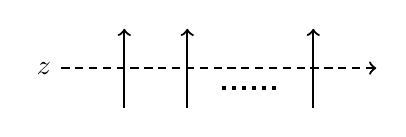
\begin{tikzpicture}[xscale=0.8, yscale=0.5, baseline=(x.base)]
    \node (x) at (0,0) {\vphantom{x}};

    \draw[thick, densely dashed, ->] (0,0) node[left] {$z$} -- (5,0);
    \draw[thick, ->] (1,-1) -- +(90:2);
    \draw[thick, ->] (2,-1) -- +(90:2);

    \draw[ultra thick, dotted, -] (2.55,-0.5) -- (3.45,-0.5);

    \draw[thick, ->] (4,-1) -- +(90:2);
  \end{tikzpicture}
  \quad .
\end{equation}
Identifying $a^{n+1} = a^1$ and taking the trace, one
obtains the \emph{transfer matrix}
$T\colon \C \to \End(\CM_{\hf^*}^{\otimes n})$:
\begin{equation}
  T(z)
  =
  \sum_{i^1, \dotsc, i^n}
  \prod_{r=1}^n
  L(z; a^r,a^{r+1})^{i^{r+1}}_{i^r}
  \prod_{s=1}^n \Delta_{i^s}^s
  \,,
  \qquad
  i^{n+1} = i^1 \,.
\end{equation}
Graphically, $T(z)$ is represented by the same picture as above but
with the horizontal direction made periodic.

By construction, $T$ is an $\End(\CM_{\hf^*}^{\otimes n})$-valued
meromorphic function.  As such, each coefficient $T_m$ in the Laurent
expansion $T(z) = \sum_{m \in \Z} T_m z^m$ is an operator acting on
the Hilbert space $\CM_{\hf^*}^{\otimes n}$.  Then, one may pick a
particular linear combination of these coefficients and declare that
it is the Hamiltonian of the quantum mechanical system.  The
Hamiltonian thus obtained is a difference operator, which is typical
of relativistic systems.

Alternatively, one may think of this system as a one-dimensional
periodic quantum spin chain.  This spin chain is constructed from $n$
solid lines extending in the longitudinal direction of a cylinder, as
shown in figure~\ref{fig:spin-chain-no-T}.  The dynamical parameter
$a^r$ resides in the region sandwiched by the $r$th and the
$(r+1)$th solid lines.  One regards the $n$ dynamical parameters
$a^1$, $\dotsc$, $a^n$ as continuous spin variables; see
figure~\ref{fig:spin-chain-chain}.  Thinking of the longitudinal
direction as the time direction, the Hilbert space of the spin chain
is again $\CM_{\hf^*}^{\otimes n}$.  An action of $T(z)$ on the
Hilbert space is induced by an insertion of a dashed line with spectral
parameter $z$ in the circumferential direction of the cylinder, as in
figure~\ref{fig:spin-chain-T}.

\begin{figure}
  \centering
  \subfloat[\label{fig:spin-chain-no-T}]{
    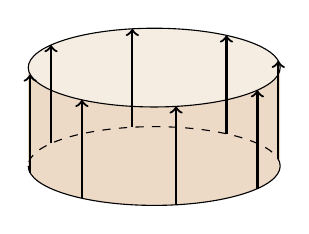
\begin{tikzpicture}[yscale=0.25, xscale=0.8]
      \fill[brown!30] (-2,0) arc (-180:0:2) -- +(0,5) arc (0:-180:2) --
      +(0,-5) -- cycle;
      \fill[brown!15]  (0,5) circle [radius=2];

      \draw[dashed] (2,0) arc (0:180:2);
      \draw (-2,0) arc (180:360:2);
      \draw (0,5) circle [radius=2];

      \draw[thick, ->] (10:2) -- ++(90:5);
      \draw[thick, ->] (55:2) -- ++(90:5);
      \draw[thick, ->] (100:2) -- ++(90:5);
      \draw[thick, ->] (145:2) -- ++(90:5);
      \draw[thick, ->] (190:2) -- ++(90:5);
      \draw[thick, ->] (235:2) -- ++(90:5);
      \draw[thick, ->] (280:2) -- ++(90:5);
      \draw[thick, ->] (325:2) -- ++(90:5);
    \end{tikzpicture}
  }
  \qquad
  \subfloat[\label{fig:spin-chain-chain}]{
    \begin{tikzpicture}[yscale=0.25, xscale=0.8]
      \draw[thick] (0,0) circle [radius=2];

      \node[spin, font=\scriptsize] at ({10-45/2}:2) {$a^3$};
      \node[spin, font=\scriptsize] at ({55-45/2}:2) {$a^4$};
      \node[spin, font=\scriptsize] at ({100-45/2}:2) {$a^5$};
      \node[spin, font=\scriptsize] at ({145-45/2}:2) {$a^6$};
      \node[spin, font=\scriptsize] at ({190-45/2}:2) {$a^7$};
      \node[spin, font=\scriptsize] at ({235-45/2}:2) {$a^8$};
      \node[spin, font=\scriptsize] at ({280-45/2}:2) {$a^1$};
      \node[spin, font=\scriptsize] at ({325-45/2}:2) {$a^2$};
    \end{tikzpicture}
  }
  \qquad
  \subfloat[\label{fig:spin-chain-T}]{
    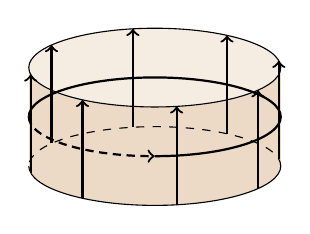
\begin{tikzpicture}[yscale=0.25, xscale=0.8]
      \fill[brown!30] (-2,0) arc (-180:0:2) -- +(0,5) arc (0:-180:2) --
      +(0,-5) -- cycle;
      \fill[brown!15]  (0,5) circle [radius=2];

      \draw[dashed] (2,0) arc (0:180:2);
      \draw (-2,0) arc (180:360:2);
      \draw (0,5) circle [radius=2];

      \draw[thick, densely dashed, ->] (-2,2.5) arc (-180:-90:2);
      \draw[thick] (-2,2.5) arc (180:-90:2);

      \draw[thick, ->] (10:2) -- ++(90:5);
      \draw[thick, ->] (55:2) -- ++(90:5);
      \draw[thick, ->] (100:2) -- ++(90:5);
      \draw[thick, ->] (145:2) -- ++(90:5);
      \draw[thick, ->] (190:2) -- ++(90:5);
      \draw[thick, ->] (235:2) -- ++(90:5);
      \draw[thick, ->] (280:2) -- ++(90:5);
      \draw[thick, ->] (325:2) -- ++(90:5);
    \end{tikzpicture}
  }
  \caption{(a) Double lines in the longitudinal direction of a
    cylinder.  (b) The corresponding quantum spin chain with
    continuous spin variables.  (c) A dashed line winding around the
    cylinder acts on the spin chain by the transfer matrix.}
  \label{fig:spin-chain}
\end{figure}

The integrability of the system is a consequence of the RLL relation.
By repeated use of the RLL relation, one deduces that the monodromy
matrix satisfies a similar relation:
\begin{equation}
  \sum_{k,l}
  R(z-z', a^{n+1})^{mn}_{kl}
  M(z)^k_i M(z')^l_j
  =
  \sum_{k,l}
  R(z-z', a^1)^{kl}_{ij}
  M(z')^n_l M(z)^m_k
  \,.
\end{equation}
Multiplying both sides by $R^{-1}(z-z', a^1)^{ij}_{mn}$, setting
$a^{n+1} = a^1$ and summing over $i$, $j$, $m$, $n$, one
finds
\begin{equation}
  T(z) T(z') = T(z') T(z) \,.
\end{equation}
In other words, transfer matrices at different values of the spectral
parameter commute.  It follows that the Laurent coefficients $\{T_m\}$
mutually commute and, in particular, commute with the Hamiltonian.
Hence, the system has a series of commuting conserved charges.

There is a slight generalization of the above construction of
commuting transfer matrices.  Suppose that $g \in \End(V)$ satisfies
\begin{equation}
  (g \otimes g) R(z,a)
  =  R(z,a) (g \otimes g)
\end{equation}
and a subspace $W$ of $V$ is invariant under $R$, $R^{-1}$, $L$ and
$g$.  (For instance, the invariance of $W$ under $R$ means that
$R(z,a)(W \otimes V) \subset W \otimes V$ and
$R(z,a)(V \otimes W) \subset V \otimes W$ for all $z$, $a$.)  Then,
the trace can be twisted by $g$ and restricted to $W$:
\begin{equation}
  T_{g,W} = \Tr_W(gM) \,.
\end{equation}
If $W_1$, $W_2$ are such invariant subspaces, then
\begin{equation}
  [T_{g,W_1}(z), T_{g,W_2}(z')] = 0 \,.
\end{equation}
Thus, we get different kinds of transfer matrices labeled by invariant
subspaces, and they commute with each other.  A typical situation in
which this construction applies is when $\hf$ is a Cartan subalgebra
of a complex Lie algebra $\gf_\C$, $V$ is a direct sum of irreducible
representations of $\gf_\C$, and $g$ is an element of $\gf_\C$.

Algebraically, L-operators give representations of \emph{dynamical
  quantum groups}~\cite{Felder:1994be, Felder:1994pb, MR1645196}.  As
an algebra, the dynamical quantum group corresponding to $R$ is
generated by the meromorphic functions on
$\C \times \hf^* \times \hf^*$, together with additional generators
$l(z)^i_j$, $l^{-1}(z)^i_j$.  The generators $l(z)^i_j$ are to be
understood as the matrix elements of an abstract L-operator and
satisfy the same relations as above; $l^{-1}(z)^i_j$ are the elements
of the inverse matrix.  This algebra has further structures (coproduct
and counit) which make it an $\hf$-bialgebroid.





\subsubsection{Elliptic L-operators}

An important example of an L-operator is one for the elliptic
dynamical R-matrix~\cite{Baxter:1972wf, MR908997, Jimbo:1987mu}, which
is a representation of the elliptic quantum group for $\slf_N$.  In
this example, $\hf$ is the Cartan subalgebra of $\slf_N$ and
$V = \C^N$ is the vector representation of $\slf_N$.

The Lie algebra $\slf_N$ consists of the traceless complex
$N \times N$ matrices and $\hf$ is the subalgebra of diagonal
elements.  We denote by $E_{ij} \in \glf_N$ the matrix that has $1$ in
the $(i,j)$th entry and $0$ elsewhere, and by $E^*_{ij}$ the element
of $\glf_N^* = \Hom(\glf_N, \C)$ such that
$\langle E_{ij}, E_{kl}^*\rangle = \delta_{ik} \delta_{jl}$.  (The
bilinear map $\langle-,-\rangle\colon \glf_N \times \glf_N^* \to \C$
is the natural pairing.)  The elements of $\hf$ are matrices of the
form $\sum_{i=1}^N b_i E_{ii}$, with $\sum_{i=1}^N b_i = 0$.  Since
$\hf$ is isomorphic to the quotient of the subspace of $\glf_N$
consisting of the diagonal matrices by the subspace spanned by the
identity matrix $I = \sum_{i=1}^N E_{ii}$, the dual space $\hf^*$ is
isomorphic to the subspace of $\glf_N^*$ consisting of elements of the
form $\sum_{i=1}^N a_i E_{ii}^*$ such that
$\langle I, \sum_{i=1}^N a_i E_{ii}^*\rangle = \sum_{i=1}^N a_i = 0$.
Thus, $\hf^*$ may also be identified with the space of traceless
diagonal matrices.

The natural action of $\slf_N$ on $\C^N$ defines the vector
representation of $\slf_N$.  In terms of the standard basis
$\{e_1, \dotsc, e_N\}$ of $\C^N$, we have
$\sum_{j=1}^N a_j E_{jj} e_i = a_i e_i$.  The weight of $e_i$ is
therefore
\begin{equation}
  h_i
  = E_{ii}^* - \frac{1}{N} \sum_{j=1}^N E_{jj}^* \,.
\end{equation}
For $a \in \hf^*$, we write $a_i = \langle E_{ii}, a\rangle$.  Then,
$\sum_{i=1}^N a_i = 0$ and
$a = \sum_{i=1}^N a_i E_{ii}^* = \sum_{i=1}^N a_i h_i$.


Fix a point $\tau$ in the upper half plane, $\Im\tau > 0$, and let
 \begin{equation}
  \theta_1(z)
  =
  - \sum_{j \in \Z + \frac12} e^{\pi\iu j^2\tau + 2\pi\iu j(z + \frac12)}
\end{equation}
be Jacobi's first theta function.  The \emph{elliptic dynamical
  R-matrix} $R^{\text{ell}}$ is defined by~\cite{Felder:1994be,
  Felder:1994pb, MR1645196}
\begin{equation}
  R^{\text{ell}}(z,a)
  =
  \sum_{i=1}^N E_{ii} \otimes E_{ii}
  + \sum_{i \neq j} \alpha(z,a_{ij}) E_{ii} \otimes E_{jj}
  + \sum_{i \neq j} \beta(z,a_{ij}) E_{ji} \otimes E_{ij}
  \,,
\end{equation}
where $a_{ij} = a_i - a_j$ and
\begin{equation}
  \alpha(z,a)
  = \frac{\theta_1(a+\eps) \theta_1(-z)}
         {\theta_1(a) \theta_1(\eps - z)} \,,
  \qquad
  \beta(z,a)
  = \frac{\theta_1(a - z) \theta_1(\eps)}
          {\theta_1(a) \theta_1(\eps - z)} \,.
\end{equation}

The \emph{elliptic L-operator} $L^{\text{ell}}$, which satisfies the
RLL relation with $R^{\text{ell}}$, has the matrix elements given
by~\cite{MR1463830}
\begin{equation}
  \label{eq:L-ell}
  L^{\text{ell}}_{w,y}(z; a^1, a^2)^j_i
  =
  \frac{\theta_1(z - w + a^2_j - a^1_i)}{\theta_1(z - w)}
  \prod_{k (\neq i)}
  \frac{\theta_1(a^1_k - a^2_j - y)}{\theta_1(a^1_{ki})}
  \,.
\end{equation}
The complex numbers $w$, $y$ may be thought of as spectral parameters
for the corresponding solid line.  The presence of the two parameters
is a consequence of the fact that $R^{\text{ell}}(z,a)$ is invariant
under shift of $a$ by a multiple of the identity matrix $I$ and in the
RLL relation~\eqref{eq:RLL} the spectral parameters $z$, $z'$ enter
the R-matrix only through the difference $z - z'$; note also that the
L-operator can be multiplied by any function of the spectral
parameter.

The elliptic dynamical R-matrix and the elliptic L-operator have many
more properties than just that they satisfy the RLL relation.  Most
importantly, the R-matrix is a solution of the dynamical Yang--Baxter
equation and encodes the Boltzmann weights for a two-dimensional
integrable lattice model.  This model is equivalent to the
eight-vertex model (or more precisely, the Belavin
model~\cite{Belavin:1981ix} which is an $\slf_N$ generalization of the
eight-vertex model~\cite{Baxter:1971cr, Baxter:1972hz}) in the sense
that the transfer matrices of the two models are related by a
similarity transformation.  The elliptic L-operator, on the other
hand, satisfies the RLL relation with another R-matrix which describes
an integrable lattice model called the Bazhanov--Sergeev
model~\cite{Bazhanov:2010kz, Bazhanov:2011mz}, whose spins variables
take values in $\hf^*$.  We will not discuss these aspects in this
paper.  The interested reader is referred to \cite{Yagi:2017hmj} for
more details.





\subsubsection{Trigonometric L-operators}


The L-operators that appear in the correspondence with Wilson--'t
Hooft lines are obtained from the elliptic L-operator $L^{\text{ell}}$
via the trigonometric limit $\tau \to \iu\infty$.  For comparison with
gauge theory results, we actually need to express these L-operators in
somewhat different forms.

First, we describe L-operators in a quantum mechanical language.  Let
us explain this description in the case in which $\hf$ is the Cartan
subalgebra of $\slf_N$.  Recall that $\slf_N$ has simple coroots
\begin{equation}
  \alpha^\vee_i = E_{ii} - E_{i+1,i+1} \,,
  \qquad
  i = 1, \, \dotsc, \, N-1 \,,
\end{equation}
and the fundamental weights
\begin{equation}
  \omega_i = (\alpha^\vee_i)^* = \sum_{j=1}^i h_j \,.
\end{equation}

Consider quantum mechanics of a particle living in
$\hf^* \times \hf^*$, with Planck constant
\begin{equation}
  \hbar = -\frac{\eps}{2\pi} \,.
\end{equation}
If $(a^1,a^2) \in \hf^* \times \hf^*$ is the position of the particle,
we write $a^r = \sum_{i=1}^{N-1} q^r_i \omega_i$, $r = 1$, $2$.
Similarly, we write the momenta $(b^1, b^2) \in \hf \times \hf$ of the
particle as $b^r = \sum_{i=1}^{N-1} p^r_i \alpha^\vee_i$.  The
corresponding position and momentum operators $\qh^r_i$, $\ph^s_i$
satisfy the canonical commutation relations:
\begin{equation}
  [\qh_i^r, \ph_j^s] = \iu\hbar \delta^{rs} \delta_{ij} \,,
  \qquad
  i, \, j = 1, \, \dotsc, \, N-1 \,.
\end{equation}
(As before, we are treating $q^r_i$, $p^r_i$ as analytically continued
variables.)

To rewrite the commutation relations in a form that is invariant under
the action of the Weyl group, we make a change of basis
\begin{equation}
  a^r = \sum_{i=1}^N a^r_i E_{ii}^* \,,
  \qquad
  b^r = \sum_{i=1}^N b^r_i E_{ii} \,.
\end{equation}
Then, the corresponding observables $\ah^r_i$, $\bh^r_i$ obey the
traceless condition,
$\sum_{i=1}^N \ah^r_i = \sum_{i=1}^N \bh^r_i = 0$, and satisfy the
commutation relations
\begin{equation}
  [\ah_i^r, \bh_j^s]
  = \iu\hbar \delta^{rs} \Bigl(\delta_{ij} - \frac{1}{N}\Bigr) \,,
  \qquad
  i, \, j = 1, \, \dotsc, \, N \,.
\end{equation}
Using these observables we can identify the matrix elements of an
L-operator $L$ with an operator in the Hilbert space of this quantum
mechanical system:
\begin{equation}
  \label{eq:L-in-QM}
  L(z)_i^j
  = L(z; \ah^1, \ah^2)_i^j e^{2\pi\iu(\bh_i^1 + \bh_j^2)} \,.
\end{equation}

In quantum mechanics, there is an invertible map from functions on the
classical phase space to operators in the Hilbert space, known as the
Weyl transform: if $q$ and $p$ are canonically conjugate variables, it
maps
\begin{equation}
  f(q,p)
  \mapsto
  \fh(\qh,\ph)
  =
  \int_{\R^4}
  \rmd x \, \rmd y \, \rmd p \, \rmd q \,
  f(q,p)
  e^{\iu(x(\qh - q) + y(\ph - p))} \,.
\end{equation}
The inverse map is the \emph{Wigner transform}, which we denote by
$\vev{-}$:
\begin{equation}
  f(\qh,\ph)
  \mapsto
  \vev{f(\qh,\ph)}
  = \int_\R \rmd x \, e^{\iu px/\hbar}
  \Bigbra{q + \frac12 x} \fh(\qh,\ph) \Bigket{q - \frac12 x} \,.
\end{equation}
In the situation at hand, if we rewrite the
expression~\eqref{eq:L-in-QM} as
\begin{equation}
  L(z)_i^j
  =
  e^{\pi\iu(\bh_i^1 + \bh_j^2)}
  \Lt(z; \ah^1, \ah^2)_i^j
  e^{\pi\iu(\bh_i^1 + \bh_j^2)}
  \,,
\end{equation}
then we have
\begin{equation}
  \vev{L(z)_i^j}
  =
  e^{2\pi\iu(b_i^1 + b_j^2)} \Lt(z; a^1, a^2)_i^j \,.
\end{equation}

Next, we apply a similarity transformation to the elliptic L-operator.
Assume $\Im\eps > 0$ and let
\begin{equation}
  \Gamma(z,\tau,\eps)
  =
  \prod_{m,n=0}^\infty
  \frac{1 - e^{2\pi\iu((m+1)\tau + (n+1)\eps - z)}}
       {1 - e^{2\pi\iu(m\tau + n\eps + z)}}
\end{equation}
be the elliptic gamma function.  Then,
$\Gammab(z) = e^{\pi\iu z^2/2\eps} \Gamma(z,\tau,\eps)$ has the
property that
$\Gammab(z + \eps, \tau,\eps) = g(\tau,\eps) \theta_1(z) \Gammab(z,
\tau,\eps)$ for some function $g(\tau,\eps)$.  We define the
conjugated L-operator $\CL^{\text{ell}}_{w,m}(z)$ by
\begin{equation}
  \CL^{\text{ell}}_{w,m}(z)_i^j
  =
  \Phi_{m-\frac12\eps}
  L^{\text{ell}}_{w,m - \frac12\eps}(z)_i^j
  \Phi_{m-\frac12\eps}^{-1} \,,
\end{equation}
where
\begin{equation}
  \Phi_y
  =
  \prod_{k,l=1}^N \Gammab(\ah^1_k - \ah^2_l - y)^{\frac12}
  \prod_{k \neq l} \Gammab(\ah^1_{kl})^{-\frac12} \,.
\end{equation}
It has the Wigner transform
\begin{multline}
  \vev{\CL^{\text{ell}}_{w,m}(z)_i^j}
  =
  e^{2\pi\iu(b_i^1 + b_j^2)}
  \frac{\theta_1(z - w + a^2_j - a^1_i)}{\theta_1(z - w)}
  \\
  \times
  \Biggl(
  \frac{\prod_{k (\neq i)} \theta_1(a^1_k - a^2_j - m)
        \prod_{l (\neq j)} \theta_1(a^1_i - a^2_l - m)}
       {\prod_{k (\neq i)}\theta_1(a^1_{ki} - \frac12\eps)
        \theta_1(a^1_{ik} - \frac12\eps)}
  \Biggr)^{\frac12}
  \,.
\end{multline}

With these preparations, let us finally take the trigonometric limit
to define the trigonometric L-operator:
\begin{equation}
  \CL_{w,m}
  = \lim_{\tau \to \iu\infty} \CL^{\text{ell}}_{w,m} \,.
\end{equation}
The trigonometric L-operator satisfies the RLL relation with the
trigonometric limit $R^{\text{trig}}$. of the elliptic R-matrix
$R^{\text{ell}}$.  Concretely, $\CL_{w,m}$ and $R^{\text{trig}}$ are
obtained from $\CL^{\text{ell}}_{w,m}$ and $R^{\text{ell}}$ by the
replacement $\theta_1(z) \to \sin(\pi z)$.

Once we are in the trigonometric setup, the quasi-periodicity in
$z \to z + \tau$ is lost and we can further take the limits
$w \to \pm\iu\infty$.  This allows us to introduce more fundamental
L-operators:
\begin{equation}
  \label{eq:fund-L}
  \CL_{\pm,m} = \lim_{w \to \pm\iu\infty} \CL_{w,m} \,.
\end{equation}
These L-operators do not depend on the spectral parameters $z$, $w$,
and their matrix elements have the Wigner transforms
\begin{equation}
  \label{eq:fund-L-ij}
  \vev{(\CL_{\pm,m})_i^j}
  =
  e^{2\pi\iu(b_i^1 + b_j^2)}
  e^{\pm\pi\iu(a^2_j - a^1_i)}
  \ell_m(a^1, a^2)_i^j \,,
\end{equation}
with
\begin{equation}
  \label{eq:ell}
  \ell_m(a^1, a^2)_i^j
  =
  \Biggl(
  \frac{\prod_{k (\neq i)} \sin\pi(a^1_k - a^2_j - m)
        \prod_{l (\neq j)} \sin\pi(a^1_i - a^2_l - m)}
       {\prod_{k (\neq i)}\sin\pi(a^1_{ki} - \frac12\eps)
        \sin\pi(a^1_{ik} - \frac12\eps)}
  \Biggr)^{\frac12}
  \,.
\end{equation}
The L-operator for arbitrary parameters $z$, $w$ can be realized as a
linear combination of $\CL_{\pm,m}$:
\begin{equation}
  \CL_{w,m}(z)
  =
  \frac{e^{\pi\iu(z-w)} \CL_{+,m} - e^{-\pi\iu(z-w)} \CL_{-,m}}{\sin\pi(z-w)}
  \,.
\end{equation}

The monodromy matrix $\CM_{\sigma,m}$ constructed from $\CL_{\pm,m}$ is
labeled by an $n$-tuple of signs
$\sigma = (\sigma^1, \dotsc, \sigma^n) \in \{\pm\}^n$ and an $n$-tuple of
complex numbers $m = (m^1, \dotsc, m^n)$:
\begin{equation}
  \label{eq:M-trig}
  \vev{(\CM_{\sigma,m})_{i^1}^{i^{n+1}}}
  =
  \sum_{i^2, \dotsc, i^n}
  \prod_{s=1}^{n+1}
  e^{2\pi\iu b^s_{i^s}}
  \prod_{r=1}^n
  e^{\sigma^r \pi\iu(a^{r+1}_{i^{r+1}} - a^r_{i^r})}
  \ell_{m^r}(a^r, a^{r+1})_{i^r}^{i^{r+1}}
  \,.
\end{equation}
The corresponding transfer matrix $\CT_{\sigma,m}$ has the Wigner transform
\begin{equation}
  \label{eq:T-trig}
  \vev{\CT_{\sigma,m}}
  =
  \sum_{i^1, \dotsc, i^n}
  \prod_{r=1}^n e^{2\pi\iu b^r_{i^r}}
  e^{\sigma^r \pi\iu(a^{r+1}_{i^{r+1}} - a^r_{i^r})}
  \ell_{m^r}(a^r, a^{r+1})_{i^r}^{i^{r+1}}
  \,,
\end{equation}
with $a^{n+1} = a^1$, $i^{n+1} = i^1$.  Our claim is that these
quantities equal the vevs of Wilson--'t Hooft lines in $\CN = 2$
supersymmetric gauge theories.





\subsection{Wilson-'t Hooft lines as transfer matrices}
\label{sec:gauge}

In the previous section we defined the fundamental trigonometric
L-operators~\eqref{eq:fund-L} and calculated transfer matrices
constructed from them.  As explained in section~\ref{sec:intro}, these
transfer matrices are expected to have interpretations as Wilson--'t
Hooft lines in $\CN = 2$ supersymmetric gauge theories described by a
circular quiver.  In this section we verify this expectation by
computing the vevs of the corresponding Wilson--'t Hooft lines.


\subsubsection{Wilson--'t Hooft lines in $S^1 \times_\epsilon \R^2 \times \R$}

Consider a four-dimensional gauge theory whose gauge group is a
compact Lie group $G$ with Lie algebra $\gf$.  Choosing a maximal
torus $T \subset G$ with Lie algebra $\tf$, we let
$\rootl(\gf) \subset \tf^*$ and $\corootl(\gf) \subset \tf$ be the
root lattice and the coroot lattice of $\gf$, respectively.  Their
duals are the coweight lattice
$\coweightl(\gf) = \rootl(\gf)^\vee \subset \tf$ and the weight
lattice $\weightl(\gf) = \corootl(\gf)^\vee \subset \tf^*$.

An 't Hooft line is the worldline of a very heavy monopole, that is, a
nondynamical magnetically charged particle.  In the presence of an 't
Hooft line, the gauge field of the theory has a singularity at the
location of the monopole: in terms of the polar angle $\theta$ and the
azimuthal angle $\phi$ of the spherical coordinates centered at the
monopole, the gauge field behaves as
\begin{equation}
  \label{eq:monopole}
  A = \frac{\mcharge}{2} (1 - \cos\theta) \rmd\phi + \dotsb \,,
\end{equation}
where $\dotsb$ represents less singular terms.  (For simplicity we are
setting the gauge theory theta angles to zero.)  The coefficient
$\mcharge$ is the magnetic charge of the monopole.  Different singular
gauge field configurations of the above form describe the same
monopole if their magnetic charges are related by gauge
transformation.  It follows that $\mcharge$ can be chosen from $\tf$,
and the choice is meaningful only up to the action of the Weyl group
$W(G)$ of $G$.

The above expression of $A$ is valid in a trivialization over a
coordinate patch that contains the point $\theta = 0$ of a two-sphere
surrounding the monopole.  At $\theta = \pi$, there is a ``Dirac
string'' which supports an unphysical magnetic flux.  For the Dirac
string to be invisible, we must have
\begin{equation}
  \langle\mcharge, w\rangle \in \Z
\end{equation}
for every weight $w \in \tf^*$ of the representation of every field in
the theory.  This is simply the condition that the holonomy of $A$
around the point $\theta = \pi$ is trivial in the bundles of which the
fields are sections.  The theory always contains fields in the adjoint
representation, so $\mcharge$ belongs to the coweight lattice:%
%
\footnote{Further, $\mcharge$ belongs to the cocharacter lattice
  $\{v \in \tf \mid \exp(2\pi\iu v) = \id_G\}$, which is a sublattice
  of $\coweightl(\gf)$.  If we take $G$ to be the adjoint group, the
  cocharacter lattice coincides with $\coweightl(\gf)$.}
%
\begin{equation}
  \mcharge \in \coweightl(\gf)/W(G) \,.
\end{equation}
Equivalently, $\mcharge$ is specified by an irreducible representation
of the Langlands dual ${}^L\gf$ of $\gf$.  In general, $\mcharge$ lies
in a sublattice of $\coweightl(\gf)/W(G)$ determined by the matter
content.

We can also consider heavy particles that carry both magnetic and
electric charges.  The worldline of such a dyon is called a Wilson--'t
Hooft line.  In the path integral formalism, a Wilson--'t Hooft line
is realized by an insertion of a Wilson line
\begin{equation}
  \label{eq:Wilson}
  \Tr_R P\exp\biggl(\iu\int_L A\biggr)
\end{equation}
and a singular boundary condition on the support $L$ of the line as
specified by the magnetic charge.  The prescribed
singularity~\eqref{eq:monopole} breaks the gauge symmetry to the
stabilizer $G_\mcharge$ of $\mcharge$, so $R$ is an irreducible
representation of $G_\mcharge$.  (More precisely, $R$ is an
irreducible representation of the stabilizer of $\mcharge$ in the
universal cover $\Gt$ of $G$~\cite{Kapustin:2005py}.)

The data specifying such a pair $(\mcharge,R)$ is actually the same as
a pair $(\mcharge, \echarge)$ of coweight $\mcharge$ and weight
$\echarge$ modulo the Weyl group action:
\begin{equation}
  (\mcharge, \echarge)
  \in
  \bigl(\coweightl(\gf) \times \weightl(\gf)\bigr)\big/W(G) \,.
\end{equation}
As emphasized in~\cite{Kapustin:2005py}, this data has more information than
a pair of irreducible representations of $\gf$ and ${}^L\gf$.

In~\cite{Ito:2011ea}, the vevs of Wilson--'t Hooft lines in $\CN=2$
supersymmetric gauge theories on $S^1 \times_\eps \R^2 \times \R$ in
the Coulomb phase were computed via localization of the path integral.
The geometry $S^1 \times_\eps \R^2$ is a twisted product of $S^1$ and
$\R^2$, constructed from $[0,2\pi r] \times \R^2$ by the
identification $(2\pi r,z) \sim (0, e^{2\pi\iu\eps} z)$, where $z$ is
the complex coordinate of $\R^2 \iso \C$.  These Wilson--'t Hooft
lines wind around $S^1$, and are located at the origin of $\R^2$ and a
point in $\R$.  In order to preserve half of the eight supercharges,
they require the complex scalar field $\phi$ in the vector multiplet
to also have a singular behavior and replace the gauge field in the
Wilson line~\eqref{eq:Wilson} with $A + \iu\Re\phi$.  The vevs depend
holomorphically on parameters
\begin{equation}
  a \in \tf_\C \,,
  \qquad
  b \in \tf^*_\C \,,
\end{equation}
which are set by the values of the gauge field and the vector
multiplet scalar at spatial infinity.  Essentially, $a$ is given by
the holonomy around $S^1$ at infinity of the gauge field, while $b$ is
that of the dual gauge field.  We refer the reader to
\cite{Ito:2011ea} for the precise definitions.

The vev of a Wilson line $W_R$ in representation $R$ is simply given
by the classical value of the holonomy:
\begin{equation}
  \label{eq:vev-W}
    \vev{W_R} = \Tr_R e^{2\pi \iu a} \,.
\end{equation}

The vevs of 't Hooft lines are much more involved.  For an 't Hooft
line $T_\mcharge$ with magnetic charge $\mcharge$, the vev takes the form
\begin{equation}
  \label{eq:vev-T}
  \vev{T_\mcharge}
  =
  \sum_{\substack{v \in \corootl(\gf) + \mcharge \\ \|v\| \leq \|\mcharge\|}}
  e^{2\pi \iu \langle v, b\rangle}
  Z_{\text{1-loop}}(a,m,\eps; v) Z_{\text{mono}}(a,m,\eps; \mcharge,v) \,,
\end{equation}
where $m$ collectively denotes complex mass parameters.  The summation
over the coweights $v$ in the shifted coroot lattice
$\corootl + \mcharge$ accounts for the so-called ``monopole
bubbling,'' a phenomenon in which smooth monopoles are absorbed by the
't Hooft line and screen the magnetic charge.  The norm $\|v\|$ with
respect to a Killing form is bounded by $\|\mcharge\|$, so this is a
finite sum.  The first two factors in the summand are the classical
action and the one-loop determinant in the screened monopole
background, respectively.  The last factor is the nonperturbative
contributions coming from degrees of freedom trapped on the 't Hooft
line due to monopole bubbling.

Suppose that the theory under consideration consists of a vector
multiplet and $N_F$ hypermultiplets in representations $R_f$ with mass
parameters $m_f$, $f = 1$, $\dotsc$, $N_F$.  The one-loop determinant
$Z_{\text{1-loop}}$ is then the product of the contributions from the
vector multiplet and the hypermultiplets:
\begin{equation}
  Z_{\text{1-loop}}(a,m,\eps; v)
  =
  Z_{\text{1-loop}}^{\mathrm{vm}}(a,\eps; v)
  \prod_{f=1}^{N_F} Z_{\text{1-loop}}^{\mathrm{hm}, R_f}(a,m_f,\eps; v) \,.
\end{equation}
The two functions are given by
\begin{align}
  Z_{\text{1-loop}}^{\mathrm{vm}}(a,\eps; v)
  &=\prod_{\alpha \in \Phi(\gf)} \prod_{k=0}^{|\langle v, \alpha\rangle| - 1}
    \sin^{-\frac12}
    \biggl(\pi\langle a, \alpha\rangle + \pi\Big(\frac12 |\langle v, \alpha\rangle| - k\Bigr)\eps\biggr) \,,
  \\
  Z_{\text{1-loop}}^{\mathrm{hm}, R}(a,m,\eps; v)
  &=\prod_{w \in P(R)}\prod_{k=0}^{|\langle v, w\rangle| - 1}
    \sin^{\frac12}\biggl(\pi \langle a, w\rangle - \pi m
    + \pi\Bigl(\frac12|\langle v, w\rangle| - \frac12 - k\Bigr)\eps\biggr) \,.
\end{align}
Here, $\Phi(\gf)$ is the set of roots of $\gf$ and $P(R)$ is the set
of weights of $R$.

The factor $Z_{\text{mono}}$ is subtle.  The original computation
in~\cite{Ito:2011ea} did not give an answer that completely matches
predictions from the AGT correspondence.  The subtleties have been
addressed in subsequent works~\cite{Brennan:2018yuj, Brennan:2018moe,
  Brennan:2018rcn, Assel:2019iae} but not resolved in full generality.

Fortunately, for Wilson--'t Hooft lines that are of interest to us,
the screened magnetic charges are in the same $W(G)$-orbit as
$\mcharge$.  The corresponding contributions are therefore obtained by
the $W(G)$-action from the perturbative term, for which $v = \mcharge$
and $Z_{\text{mono}} = 1$.

To our knowledge, a formula for the vevs of dyonic Wilson--'t Hooft
lines generalizing the expressions~\eqref{eq:vev-W}
and~\eqref{eq:vev-T} has not been derived.  Nevertheless, for the same
reason as mentioned, we can calculate the vev of a relevant Wilson--'t
Hooft line by first writing down its perturbative contribution, which
is simply the product of the perturbative vevs of the corresponding
purely electric and purely magnetic lines, and then summing over the
contributions from the nonperturbative sectors related by the
$W(G)$-action.





\subsubsection{Transfer matrices from circular quiver theories}
\label{sec:circular-quiver-theory}

The Wilson--'t Hooft line that corresponds to the transfer
matrix~\eqref{eq:T-trig} is one in an $\CN = 2$ supersymmetric gauge
theory that is described by a circular quiver with $n$ nodes:
\begin{equation}
  \begin{tikzpicture}[scale=0.8, baseline=(x.base)]
    \node (x) at (0,0) {\vphantom{x}};

    \draw[dotted] (163:1) arc (163:197:1);
    \draw (-155:1) arc (-155:155:1);

    \node[gnode] at (0:1) {$N$};
    \node[gnode] at (60:1) {$N$};
    \node[gnode] at (120:1) {$N$};
    \node[gnode] at (240:1) {$N$};
    \node[gnode] at (300:1) {$N$};
  \end{tikzpicture}
  \quad .
\end{equation}
Each node represents a vector multiplet for an $\SU(N)$ gauge group,%
%
\footnote{More precisely, the gauge group is a product of $\PSU(N)$.}
%
and each edge a hypermultiplet that transforms in the bifundamental
representation under the gauge groups of the nodes it connects.

Let us first consider the case in which the quiver consists of a
single node and a single edge.  In this case, the gauge group
$G = \SU(N)$ and the only hypermultiplet is in the adjoint
representation.  This theory is known as $\CN = 2^*$ theory.

The roots of $\gf = \suf_N$ are
$\alpha_{ij} = E_{ii}^* - E_{jj}^* = h_i - h_j$, $i \neq j$.  The
positive roots are $\alpha_{ij}$, $i < j$, and the simple roots are
$\alpha_i = \alpha_{i,i+1}$, $i = 1, \,, \dotsc,\, N-1$.  The
fundamental coweights are
$\omega^\vee_i = (\alpha_i^\vee)^* = \sum_{j=1}^i h^\vee_j$, with
\begin{equation}
  h^\vee_i = E_{ii} - \frac{1}{N} \sum_{j=1}^N E_{jj} \,.
\end{equation}
The various lattices are
\begin{equation}
  \rootl = \bigoplus_{i=1}^{N-1} \Z \alpha_i \,,
  \qquad
  \corootl = \bigoplus_{i=1}^{N-1} \Z \alpha^\vee_i \,,
  \qquad
  \weightl = \bigoplus_{i=1}^{N-1} \Z \omega_i \,,
  \qquad
  \coweightl = \bigoplus_{i=1}^{N-1} \Z \omega^\vee_i \,.
\end{equation}
We recall that $\alpha^\vee_i$ are the simple coroots and
$\omega_i = (\alpha^\vee_i)^*$ are the fundamental weights.


% An element of the Cartan subalgerbra $\tf$ of $\suf_N$ can be
% written as a real linear combination $\sum_{k=1}^N a_k E_{kk}$ such
% that $\sum_{k=1}^N a_k = 0$.  Since
% $[\sum_{k=1}^N a_k E_{kk}, E_{ij}] = (a_i - a_j) E_{ij}$, the roots
% of $\suf_N$ are $\alpha_{ij} = E_{ii}^\vee - E_{jj}^\vee$.  The
% positive roots are $\alpha_{ij}$, $i < j$.  The simple roots are
% \begin{equation}
%   \alpha_i = \alpha_{i,i+1} = h_i - h_{i+1} \,,
%   \qquad
%   i = 1, \,, \dotsc,\, N-1 \,.
% \end{equation}
% The simple roots form a basis of $\tf^*$.

% The elements $\alpha^\vee_{\alpha_{ij}} = E_{ii} - E_{jj}$,
% $E_{\alpha_{ij}} = E_{ij}$ and $E_{-\alpha_{ij}} = E_{ji}$ satisfy the
% relations
% $[\alpha^\vee_{\alpha_{ij}}, E_{\pm\alpha_{ij}}] = \pm 2E_{\pm\alpha_{ij}}$ and
% $\alpha^\vee_{\alpha_{ij}} = [E_{\alpha_{ij}}, E_{-\alpha_{ij}}]$, showing that
% $\alpha^\vee_{\alpha_{ij}}$, $i \neq j$, are the coroots of $\suf_N$.  The
% simple coroots
% \begin{equation}
%   \alpha^\vee_i
%   = \alpha^\vee_{\alpha_i}
%   = E_{ii} - E_{i+1,i+1} \,,
%   \qquad
%   i = 1, \, \dotsc, \, N-1 \,,
% \end{equation}
% span $\tf$.  The dual basis vectors of $\tf^*$,
% \begin{equation}
%   \omega_i
%   = \alpha^\vee_i^\vee
%   = \sum_{j=1}^i h_i \,,
% \end{equation}
% are the fundamental weights of $\suf_N$.  An element
% $\lambda \in \tf^*$ is the highest weight of an irreducible
% representation of $\suf_N$ if and only if
% $\lambda = \sum_{i=1}^{N-1} n_i \omega_i$ for some integers
% $n_i \geq 0$.


% We take the gauge group $G = \U(1) \times \SU(N)^n$, where the $\U(1)$
% factor is the diagonal subgroup of $\U(N)^n$ in which $\SU(N)^n$ is
% naturally embedded.  The $\U(1)$ factor is important for us to
% construct relevant Wilson--'t Hooft lines, but does not really show up
% in the computation.


% The elements of the cocharacter lattice of $G$ are real diagonal
% matrices of the form
% \begin{equation}
%   \sum_{r=1}^n \sum_{i=1}^N (B_0 + B^r_i) E_{ii}^r \,,
%   \qquad
%   B_0 \,, B^r_i \in \R \,,
% \end{equation}
% such that
% \begin{equation}
%   \sum_{i=1}^N B^r_i = 0 \,,
%   \qquad
%   B_0 + B^r_i \in \Z \,.
% \end{equation}
% Here, $E_{ii}^r$ is the matrix $E_{ii}$ regarded as a generator of the
% $r$th $\U(N)$ factor.  Such a matrix is specified by an $n$-tuple of
% $N$-tuples of integers
% \begin{equation}
%   (m^1, \dotsc, m^n) \in \Z^{nN} \,,
%   \qquad
%   m^r \in \Z^N \,,
% \end{equation}
% such that
% \begin{equation}
%   \sum_{i=1}^N m^r_i = \sum_{i=1}^N m^s_i
% \end{equation}
% for all $r$, $s$.  Concretely, $B_0 = \sum_i m^r_i/N$ and
% $B^r_i = m^r_i - B_0$.


For $\CN = 2^*$ theory with $G = \SU(N)$, minimal magnetic charges are
$\mcharge = \omega^\vee_1 = h^\vee_1$ and
$\mcharge = \omega^\vee_{N-1} = -h^\vee_N$.  These magnetic charges are the
highest weights of the fundamental representation and the
antifundamental representation of ${}^L\suf_N \iso \suf_N$,
respectively.

Let us consider the 't Hooft line with $\mcharge = h^\vee_1$.  The vev
of this 't Hooft line is expressed as a sum over the screened magnetic
charges $v = h^\vee_1$, $h^\vee_2$, $\dotsc$, $h^\vee_N$.  The term
for $v = h^\vee_1$ is the perturbative contribution and given by
\begin{equation}
  e^{2\pi\iu b_1}
  \prod_{j=2}^N
  \sin^{-\frac12}\Bigl(\pi a_{1j} + \frac12 \pi\eps\Bigr)
  \sin^{-\frac12}\Bigl(\pi a_{j1} + \frac12 \pi\eps\Bigr)
  \sin^{\frac12}(\pi a_{1j} - \pi m)
  \sin^{\frac12}(\pi a_{j1} - \pi m) \,,
\end{equation}
where $a_i = \langle a, h_i\rangle$,
$b_i = \langle h^\vee_i, b\rangle$, $a_{ij} = a_i - a_j$ and $m$ is
the mass of the adjoint hypermultiplet.  The other terms are related
to this perturbative term by the Weyl group action which permutes
$(h^\vee_1, \dotsc, h^\vee_N)$, so we find
\begin{equation}
  \vev{T_{h^\vee_1}}
  =
  \sum_{i=1}^N
  e^{2\pi\iu b_i}
  \prod_{j (\neq i)}
  \biggl(
  \frac{\sin\pi(a_{ij} - m) \sin\pi(a_{ji} - m)}
       {\sin\pi(a_{ij} - \frac12\eps) \sin\pi(a_{ji} - \frac12\eps)}
  \biggr)^{\frac12} \,.
\end{equation}
The vev of $T_{-h^\vee_N}$ is obtained from $\vev{T_{h^\vee_1}}$ by
the replacement $b_i \to -b_i$.

% An important fact shown in \cite{Ito} is that the vevs of the 't Hooft
% loops satisfy the Moyal product. One can observe that, for example\footnote{The second relation of the Moyal product may have an ambiguity. The
% left hand side should depend on the ordering of the product. This
% might stems from the monopole screening contribution, but again we
% do not discuss this point. }
% \begin{equation}
% \left\langle T_{B=(1,0^{N-1})}\right\rangle *\left\langle T_{B=(1,0^{N-1})}\right\rangle
%   =\left\langle T_{B=(2,0^{N-1})}\right\rangle ,
% \end{equation}
%  and
% \begin{equation}
% \left\langle T_{B=(-1,0^{N-1})}\right\rangle *\left\langle T_{B=(1,0^{N-1})}\right\rangle
%   =\left\langle T_{B=(1,-1,0^{N-2})}\right\rangle ,
% \end{equation}
% i.e. the OPE of the 't Hooft loops in the path integral defines the
% Moyal product between the vev of the loops. This Moyal product is
% associated with the Poisson structure determined by the holomorphic
% symplectic form
% \begin{equation}
% da\wedge db:=\sum_{i}da_{i}\wedge db_{i},
% \end{equation}
%  and defined by
% \begin{equation}
% (f*g)(a,b)
%   :=e^{i\frac{\eps}{4\pi}(\partiah^\vee_{b}\cdot\partiah^\vee_{a^{\prime}}-\partiah^\vee_{a}\cdot\partiah^\vee_{b^{\prime}})}
%   f(a,b)g(a^{\prime},b^{\prime})\mid_{a^{\prime}\rightarrow a,b^{\prime}\rightarrow b}.
% \end{equation}
% The fact that the vev of the 't Hooft loops satisfies the Moyal product
% means that they realize the deformation quantization of the Coulomb
% branch and it is natural for the vev of 't Hooft operators to be Weyl
% transformed into a difference operator acting on some Hilbert space;
% the Moyal product turns out to be an operator product. The difference
% operator obtained from the 't Hooft loop in $\CN=2^{*}$ theory
% on $S^{1}\times\R^{3}$ is actually identified with the trigonometric
% version of the Ruijsenaars' operator \cite{Has}. From these observations
% we may expect that the algebra of the 't Hooft loops defined by the
% Moyal product is isomorphic to the algebra of difference operators
% in a corresponding integrable lattice model. As we will see, through
% AGT correspondence the difference operators in general can be identified
% with the Verlinde operators acting on the space of conformal blocks
% in Toda conformal field theory.


Now, let us turn to a circular quiver with $n$ nodes.  For this
theory, we have $G = \SU(N)^n$ and
$\coweightl(\gf) = \coweightl(\suf_N)^{\oplus n}$.  We consider the 't
Hooft line with
\begin{equation}
  \label{eq:B-circular}
  \mcharge =  h^\vee_1 \oplus \dotsb \oplus h^\vee_1 \,,
\end{equation}
charged equally under the $\SU(N)$ factors of $G$.  This time, the
summation is over all coweights of the form
$v = h^\vee_{i^1} \oplus \dotsb \oplus h^\vee_{i^n}$.  The perturbative term,
for which $i^1 = \dotsb = i^n = 1$, is given by
\begin{multline}
  \label{eq:T-circ-pert}
  \prod_{r=1}^n
  e^{2\pi\iu b^r_1}
  \prod_{j=2}^N
  \sin^{-\frac12}\Bigl(\pi a^r_{1j} + \frac12 \pi\eps\Bigr)
  \sin^{-\frac12}\Bigl(\pi a^r_{j1} + \frac12 \pi\eps\Bigr)
  \\
  \times
  \sin^{\frac12}\bigl(\pi(a^r_j - a^{r+1}_1) - \pi m^r \bigr)
  \sin^{\frac12}\bigl(\pi(a^r_1 - a^{r+1}_j) - \pi m^r\bigr)
  \,.
\end{multline}
The superscript $r$ refers to the $r$th $\SU(N)$ factor of $G$, with
$a^{n+1} = a^1$.  Collecting the contributions from the other
coweights, we get
\begin{equation}
  \vev{T_{h^\vee_1 \oplus \dotsb \oplus h^\vee_1}}
  =
  \sum_{i^1, \dotsc, i^n}
  \prod_{r=1}^n
  e^{2\pi\iu b^r_{i^r}}
  \ell_{m^r}(a^r, a^{r+1})_{i^r}^{i^{r+1}} \,,
\end{equation}
where we have used the functions~\eqref{eq:ell}.

Comparing this expression with the Wigner transform~\eqref{eq:T-trig}
of the trigonometric transfer matrix $\CT_{\sigma,m}$, we see
\begin{equation}
  \vev{T_{h^\vee_1 \oplus \dotsb \oplus h^\vee_1}}
  =
  \vev{\CT_{(+,\dotsc,+), m}}
  =
  \vev{\CT_{(-,\dotsc,-), m}}
\end{equation}
under the obvious identification of parameters.

In order to reproduce $\vev{\CT_{\sigma,m}}$ for a general choice of
the signs $\sigma$, we add to the 't Hooft line the electric charge
\begin{equation}
  \label{eq:E-circular}
  \echarge
  = \sum_{r=1}^n \sigma^r \frac12(h^{r+1}_1 - h^r_1)
  = \sum_{r=1}^n (\sigma^r 1 - \sigma^{r+1} 1)  \frac12 h^{r+1}_1 \,.
\end{equation}
This electric charge is in a sense a minimal one that is compatible
with the Dirac--Schwinger--Zwanziger quantization condition for
locality: the charges $(\mcharge,\echarge)$ and
$(\mcharge',\echarge')$ of two dyons must satisfy
$\langle \mcharge, \echarge'\rangle - \langle \mcharge',
\echarge\rangle \in \Z$.  In section~\ref{sec:Toda}, we will see the
geometric meaning of this ``minimality'' in connection with the AGT
correspondence.

The magnetic charge~\eqref{eq:B-circular} breaks the gauge group to
$\mathrm{S}(\U(1) \times \U(N-1))^n$, and we are turning on a Wilson
line that is charged under the $\U(1)$ factors with charges
proportional to $(\sigma^r 1 - \sigma^{r+1} 1)/2$.  The Wilson line
multiplies the perturbative term~\eqref{eq:T-circ-pert} by the phase
factor
\begin{equation}
  \prod_{r=1}^n e^{\sigma^r \pi\iu \langle a, h^{r+1}_1 - h^r_1\rangle}
  =
  \prod_{r=1}^n e^{\sigma^r \pi\iu (a^{r+1}_1 - a^r_1)} \,.
\end{equation}
Hence, the term with $v = h^\vee_{i^1} \oplus \dotsb \oplus h^\vee_{i^n}$ gets
the phase factor
$e^{\sigma^r \pi\iu (a^{r+1}_{i^{r+1}} - a^r_{i^r})}$, and the vev of
this Wilson--'t Hooft line matches the Wigner transform of
$\CT_{\sigma,m}$.



\subsubsection{Monodromy matrices from linear quiver theories}

We have considered the Wilson--'t Hooft lines in the circular quiver
theory and showed that their vevs match the Wigner transforms of the
trigonometric transfer matrices.  What correspond to the monodromy
matrices then?  In view of the fact that summing over the weights of
the representation $V = \C^N$ in the integrable model amounts to
summing over the different screened magnetic charges, natural
candidates are Wilson--'t Hooft lines in a theory described by a
linear quiver with $n + 1$ nodes:
\begin{equation}
  \label{eq:linear-q}
  \begin{tikzpicture}[baseline=(x.base)]
    \node (x) at (0,0) {\vphantom{x}};

    \node[fnode] (1) at (0,0) {$N$};
    \node[gnode] (2) at (1,0) {$N$};
    \node[gnode] (3) at (2,0) {$N$};
    \node[gnode] (n) at (3.6,0) {$N$};
    \node[fnode] (n+1) at (4.6,0) {$N$};

    \draw (1) -- (2) -- (3) -- +(0:0.5);
    \draw[dotted] (2.5,0) -- (3.1,0);
    \draw (n) -- +(180:0.5);
    \draw (n) -- (n+1);
  \end{tikzpicture}
  \quad .
\end{equation}
The leftmost and the rightmost nodes represent $\SU(N)$ flavor groups,
which are not gauged.

In particular, we expect that the fundamental trigonometric
L-operators~\eqref{eq:fund-L} arise from the vevs of Wilson--'t Hooft
lines of the theory of a bifundamental hypermultiplet:
\begin{equation}
  \label{eq:two-node-q}
  \begin{tikzpicture}[baseline=(x.base)]
    \node (x) at (0,0) {\vphantom{x}};

    \node[fnode] (1) at (0,0) {$N$};
    \node[fnode] (2) at (1,0) {$N$};
    \draw (1) -- (2);
  \end{tikzpicture}
  \quad .
\end{equation}
Let us see if this is the case.

We introduce nondynamical vector multiplets for the $\SU(N)$ flavor
groups, and consider the Wilson--'t Hooft lines with magnetic charge
\begin{equation}
  \mcharge = h^\vee_i \oplus h^\vee_j
\end{equation}
and electric charges
\begin{equation}
  \echarge =  \mp\frac12 h_i \oplus \pm\frac12 h_j\,.
\end{equation}
Note that the electric charges are fractional.  The vevs of these
Wilson--'t Hooft lines are
\begin{equation}
  e^{2\pi\iu (b^1_i + b^2_j)}
  e^{\pm\pi\iu (a^2_j - a^1_i)}
  \prod_{k (\neq i)}
  \prod_{l (\neq j)}
  \bigl(\sin\pi(a^1_k - a^2_j - m)
  \sin\pi(a^1_i - a^2_l - m)\bigr)^{\frac12} \,.
\end{equation}
The vevs do not quite match the Wigner transforms~\eqref{eq:fund-L-ij}
of $(\CL_{\pm,m})_i^j$.  They differ by the factor in the denominator
of the function~\eqref{eq:ell}.

This factor is the one-loop determinant associated with the first
node; it would have been present had the $\SU(N)$ flavor group been
gauged and the vector multiplet been dynamical.  From the gauge theory
point of view, it is natural to think of this factor as a weight
accompanying the summation over the screened magnetic charges.  On the
integrable system side, we could as well omit the denominator in
question from the definitions of the L-operators and adopt the
convention that the same weight is included when operators are
multiplied within $V$.  The L-operators would still satisfy the RLL
relation.

To get the monodromy matrix~\eqref{eq:M-trig}, we take $n$ L-operators
and multiply them inside $V$.  The gauge theory counterpart of this
operation is to connect $n$ copies of the two-node
quiver~\eqref{eq:two-node-q}, in the presence of appropriate
Wilson--'t Hooft lines of the type considered above, by identifying
and gauging flavor nodes.  This produces the $n+1$ node linear
quiver~\eqref{eq:linear-q} and the Wilson--'t Hooft lines with
magnetic charge
\begin{equation}
  \label{eq:B-linear}
  \mcharge
  =
  h^\vee_{i^1} \oplus h^\vee_1 \oplus h^\vee_1 \oplus \dotsb \oplus h^\vee_1
  \oplus h^\vee_{i^{n+1}}
\end{equation}
and electric charge
\begin{equation}
  \echarge
  =
  \sigma^1 \frac12 (h_1^2 - h_{i^1}^1)
  + \sum_{r=2}^{n-1} \sigma^r \frac12 (h^{r+1}_1 - h^r_1)
  + \sigma^n \frac12 (h_{i^{n+1}}^{n+1} - h_1^n) \,.
\end{equation}
The vev of this Wilson--'t Hooft line reproduces the Wigner
transform~\eqref{eq:M-trig}, except that a factor corresponding to the
one-loop determinant for the vector multiplet for the first node is
missing.



\subsubsection{Other representations}

The magnetic charge~\eqref{eq:B-circular} of the above Wilson--'t
Hooft lines is the highest weight of the representation
$(\C^N)^{\oplus n}$ of the Langlands dual
${}^L\gf_\C \iso \slf_N^{\oplus n}$ of $\gf_\C$.  The corresponding
transfer matrix~\eqref{eq:T-trig} is represented graphically as $n$
solid lines intersected by a single dashed loop carrying the
representation $V = \C^N$, as shown in figure~\ref{fig:spin-chain-T}.
The $n$ regions sandwiched between solid lines correspond to the $n$
copies of $\slf_N$.

Both sides of the correspondence have a generalization in which the
vector representation $\C^N$ is replaced by another representation $R$
of $\slf_N$.  On the gauge theory side, we can change the magnetic
charge of the Wilson--'t Hooft lines to the highest weight $\lambda_R$
of $R^{\oplus n}$ while keeping the electric charges intact.  On the
integrable system side, the counterpart of this operation is the
fusion procedure, which allows one to construct a dashed line in an
arbitrary finite-dimensional representation of $\slf_N$ from a
collection of dashed lines in the vector representation, with the
spectral parameters suitably adjusted.

We naturally expect that the vev of the Wilson--'t Hooft line with
magnetic charge $\mcharge = \lambda_R^{\oplus n}$ is equal to the
Wigner transform of a transfer matrix constructed from L-operators in
representation $R$, obtained by fusion from the
L-operators~\eqref{eq:fund-L} in the vector representation.

For $n = 1$ and $R = \wedge^k \C^N$, this equality can be verified
from known results.  In this case, the transfer matrix is the
trigonometric limit of Ruijsenaars' difference
operator~\cite{Ruijsenaars:1986pp}
\begin{equation}
  \sum_{\substack{I \subset \{1, \dotsc, N\} \\ |I| = k}}
  \Delta_I^{\frac12}
  \prod_{\substack{i \in I \\ j \notin I}}
  \sqrt{
    \frac{\theta_1(a_{ji} - m) \theta_1(a_{ij} - m)}
         {\theta_1(a_{ji} - \frac12 \eps) \theta_1(a_{ij} - \frac12 \eps)}
  }
  \Delta_I^{\frac12} \,,
  \qquad
  \Delta_I = \prod_{i \in I} \Delta_i \,,
\end{equation}
and is related to the Macdonald operator by a similarity
transformation~\cite{MR1463830}.  On the other hand, the exterior
power $\wedge^k \C^N$ being a minuscule representation (that is, all
weights are related by the action of the Weyl group), the vev of the
't Hooft line with
$\mcharge = \omega^\vee_k = h^\vee_1 + \dotsb + h^\vee_k$ in
$\CN = 2^*$ theory can be computed from the perturbative term:
\begin{equation}
  \vev{T_{\omega^\vee_k}}
  =
  \sum_{\substack{I \subset \{1, \dotsc, N\} \\ |I| = k}}
  \prod_{\substack{i \in I \\ j \notin I}}
  e^{2\pi\iu b_i}
  \biggl(
  \frac{\sin\pi(a_{ij} - m) \sin\pi(a_{ji} - m)}
       {\sin\pi(a_{ij} - \frac12\eps) \sin\pi(a_{ji} - \frac12\eps)}
  \biggr)^{\frac12} \,.
\end{equation}
(For $\CN = 2^*$ theory the choice of the signs $\sigma = \pm$ is
irrelevant.)  The vev matches the Wigner transform of the
trigonometric Ruijsenaars operator.

In the case of symmetric powers, we find a discrepancy between this
proposal and the formula~\eqref{eq:vev-T}.  The vev of the 't Hooft
line with $\mcharge = kh^\vee_1$ in $\CN = 2^*$ theory, as computed by
that formula, can be expressed as the Moyal product of $k$ copies of
the vev for the vector representation~\cite{Ito:2011ea,
  Hayashi:2019rpw}:
\begin{equation}
  \vev{T_{kh^\vee_1}}
  = \vev{T_{h^\vee_1}} \star \dotsb \star \vev{T_{h^\vee_1}} \,.
\end{equation}
The Moyal product $\star$ has the property that
$\vev{f} \star \vev{g} = \vev{fg}$ with respect to the Wigner
transform, so this equation means that we have
\begin{equation}
  \vev{T_{kh^\vee_1}} = \vev{\CT_m^k} \,.
\end{equation}
However, $\CT_m^k$ is the transfer matrix in the tensor product
representation $(\C^N)^{\otimes k}$, not the $k$th symmetric power of
$\C^N$.  The discrepancy might be ascribed to subtle monopole
contributions to the vev of the 't Hooft line.





\subsection{Transfer matrices from Verlinde operators}
\label{sec:Toda}


%%%%%  AGT  %%%%%
Here we briefly review  the role of line and surface operators
in the AGT correspondence. Let us first give the general statements
of the correspondence and the notion of class $\CS$ theories,
which already appeared in section \ref{sec:surface_defects}.
For more details, see excellent reviews \cite{LeFloch:2020uop,Okuda:2014fja,Gukov:2014gja}
and the references therein.

The AGT correspondence was found heuristically by Alday,
Gaiotto and Tachikawa \cite{Alday:2009aq}, based on the observations
made in \cite{Gaiotto:2009we}. It was derived basically by comparing
the instanton partition function \cite{Nekrasov:2002qd} of the $\CN =2$ SU$(2)$
gauge theory with the Liouville conformal block.
Soon after their work, many checks and generalizations have been made, and
it has been known that the statement applies to the correspondence between a large class
 of four-dimensional $\CN = 2$ supersymmetric gauge theories on four-manifold $M^4$,
 which is now called the theories of class $\CS$, labeled by punctured Riemann
surfaces $C_{g,n}$ and two-dimensional non-supersymmetric QFTs defined on the Riemann surfaces.

The origin of the AGT correspondence is the six-dimensional $(2,0)$ SCFT. Let the four-manifold $M^4$ be
$\R^4_{\eps_1,\eps_2}$ (or $S^4_{\eps_1,\eps_2}$). Then this higher dimensional
theory explains the correspondence such that the two theories are originally a single theory in six dimensions:
\begin{equation}
    \def\height{1.2cm}
        \begin{tikzpicture}[scale=1.0, baseline=(x.base)]    \node (x) at (0,\height/2) {\vphantom{x}};

        \node (dummy) at (0,0) {};
        \node[above=\height of dummy, align=center] (6d) {6d theory \\ on $M^4\times C_{g,n}$};
        \node[left=1cm of dummy, align=center] (4d) {4d $\CN =2$ gauge theory \\ on $M^4$};
        \node[right=1cm of dummy, align=center] (2d) {2d Liouville/Toda CFT \\ on $C_{g,n}$};

        \draw[semithick, arrows=-to] (6d) -- (4d);
        \draw[semithick, arrows=-to] (6d) -- (2d);

    \end{tikzpicture}
\end{equation}
where
%the four-dimensional theory is defined on a four-manifold $M^4=\R^4_{\eps_1,\eps_2}$
%(or $S^4_{\eps_1,\eps_2}$).
$\eps_1$ and $\eps_2$ are
called $\Omega$-deformation parameters in the literature, which turn out
to realize the deformation quantization of the moduli spaces.
For $M^4=\R^4_{\eps_1,\eps_2}$, the $\Omega$-deformation causes
two-dimensional rotations on the planes $\mathbb R^2_{\eps_1}$ and $\mathbb R^2_{\eps_2}$:
\begin{equation}
    \R^4_{\eps_1,\eps_2} := \R^2_{\eps_1} \times \R^2_{\eps_2}.
\end{equation}
Hence, the $\Omega$-deformation breaks the whole rotation symmetry $\mathrm{SO}(4)$ of $\mathbb R^4$ to
its subgroup $\SO(2)_{\eps_1}\times\SO(2)_{\eps_2}$.
$\Omega$ deformation leads to the Gaussian regularization of $\mathbb R^4$ and $\mathbb R^2$,
and their infinite volumes are regularized such that
\begin{equation}
    \rm{Vol}\left(  \R^4_{\eps_1,\eps_2}  \right) = \int_{\R^4_{\eps_1,\eps_2}}1 = \frac{1}{\eps_1 \eps_2} ,
    \qquad  \rm{Vol}\left(  \R^2_{\eps}  \right) = \int_{\R^2_{\eps}}1 = \frac{1}{\eps}
\end{equation}
Such a twist allows us to calculate quantities that are invariant under the $\U(1) \simeq \SO(2)$
action on each plane, using the Duistermaat-Heckman fixed point formula
\cite{Duistermaat:1982vw} (or more generally Atiyah-Bott localization formula \cite{Atiyah:1984px}).
Nekrasov applied these techniques to compute instanton partition function, which is an integral over
the instanton moduli space, and obtained the exact results \cite{Nekrasov:2002qd,Nekrasov:2003rj}
which plays a crucial role in the AGT correspondence.


%%%%%  AGT  %%%%%





\subsubsection{Review of AGT correspondence}

We have computed the vevs of a class of Wilson--'t Hooft lines in
$\CN = 2$ supersymmetric gauge theories described by a circular
quiver, and found that they match the Wigner transforms of transfer
matrices constructed from the fundamental trigonometric L-operators.
In this section, we show that these transfer matrices can also be
identified with Verlinde operators in Toda theory on a punctured
torus.  The result is in keeping with the relation proposed
in~\cite{Ito:2011ea} based on the AGT
correspondence~\cite{Alday:2009aq} between Toda theory and $\CN = 2$
supersymmetric field theories.




The AGT correspondence originates from six-dimensional $\CN = (2,0)$
supersymmetric field theory, of type $A_{N-1}$ in our case, placed on
$S^4_\bs \times C_{g,n}$.  Here, $S^4_\bs$ is an ellipsoid, defined as
a submanifold of $\R^5$ by the equation
\begin{equation}
  (x^1)^2
  + \bs^{-2} \bigl((x^2)^2 + (x^3)^2\bigr)
  + \bs^2 \bigl((x^4)^2 + (x^5)^2\bigr)
  = r^2 \,,
\end{equation}
and $C_{g,n}$ is a Riemann surface of genus $g$ with $n$ punctures.
With partial topological twisting along $C_{g,n}$, this system
preserves eight of the sixteen supercharges of $\CN = (2,0)$
supersymmetry in six dimensions.

In the limit in which $C_{g,n}$ shrinks to a point, the
six-dimensional theory reduces to a four-dimensional $\CN = 2$
supersymmetric field theory on $S^4_\bs$, whose gauge and matter
contents are determined by the choice of a pants decomposition of
$C_{g,n}$ and boundary conditions at the
punctures~\cite{Gaiotto:2009we, Gaiotto:2009hg}.  The theories
discussed in section~\ref{sec:gauge} can all be obtained in this way.
If one instead integrates out the modes along $S^4_\bs$, one is left
with $A_{N-1}$ Toda theory on $C_{g,n}$ with central charge
\begin{equation}
  c = 1 + 6q^2 \,,
  \qquad
  q = \bs + \bs^{-1} \,,
\end{equation}
with vertex operators $V_{\beta^r}$, $r = 1$, $\dotsc$, $n$, inserted
at the punctures.  According to the AGT correspondence, the partition
function of the theory on $S^4_\bs$ equals the correlation function of
Toda theory on $C_{g,n}$:
\begin{equation}
  \vev{1}_{S^4_\bs} = \biggvev{\prod_r V_{\beta^r}}_{C_{g,n}} \,.
\end{equation}

Let the vertex operators at the punctures be primary fields
$V_{\beta^r}$, $r = 1$, $\dotsc$, $n$, labeled by momenta
$\beta^r \in \hf^*$ valued in the dual of the Cartan subalgebra $\hf$
of $\slf_N$.  Given a pants decomposition of $C_{g,n}$, the Toda
correlation function takes the form
\begin{equation}
  \biggvev{\prod_r V_{\beta^r}}_{C_{g,n}}
  =
  \int [\rmd\alpha] \,
  \CC(\alpha; \beta)
  \overline{\CF(\alpha; \beta)} \CF(\alpha; \beta) \,,
\end{equation}
where $[\rmd\alpha]$ is a measure of integration over the set
$\alpha = \{\alpha^1, \dotsc, \alpha^{3g - 3 + n}\}$ of momenta
assigned to the internal edges of the pants decomposition,
$\beta = \{\beta^1, \dotsc, \beta^n\}$ is the set of momenta assigned
to the external edges, $\CC(\alpha; \beta)$ is the product of relevant
three-point functions, and $\CF(\alpha; \beta)$ is the corresponding
conformal block which is a meromorphic function of $\alpha$ and
$\beta$.

On the gauge theory side, $\CC(\alpha; \beta)$ is interpreted as the
product of the classical and the one-loop contributions to the
partition function on $S^4_\bs$, whereas $\CF(\alpha; \beta)$ and
$\overline{\CF(\alpha; \beta)}$ represent the nonperturbative
contributions from instantons localized at the two poles at
$x^2 = x^3 = x^4 = x^5 = 0$.  The internal momenta $\alpha$ are
related to the zero modes $\as$ of scalar fields in the vector
multiplets by
\begin{equation}
  \alpha = Q + \iu\as \,,
\end{equation}
and the external momenta $\beta$ are identified with mass parameters
for matter multiplets.






\subsubsection{Verlinde operators and Wilson--'t Hooft lines}

To incorporate Wilson--'t Hooft lines in the gauge theory, one
introduces Verlinde loop operators in the Toda theory.  We will
explain the construction of relevant Verlinde operators in concrete
examples.  For the moment, it suffices to say that they are specified
by a momentum of the form $\mu = -\bs\lambda$ and a one-cycle $\gamma$
in $C_{g,n}$, where $\lambda$ is the highest weight of a
representation of $\slf_N$.%
%
\footnote{More generally, the momentum takes the form
  $\mu = -\bs\lambda_1 - \bs^{-1} \lambda_2$, where $\lambda_1$,
  $\lambda_2$ are the highest weights of a pair of representations of
  $\slf_N$.  The corresponding Wilson--'t Hooft line is a
  superposition of lines wrapping $S^1_\bs$ and another circle
  $S^1_{\bs^{-1}}$ where $x^2 = x^3 = 0$.}
%
In the presence of a Verlinde operator $\Phi_\mu(\gamma)$, the Toda
correlation function is modified to
\begin{equation}
  \biggvev{\Phi_\mu(\gamma) \prod_r V_{\beta^r}}_{C_{g,n}}
  =
  \int [\rmd\alpha] \,
  \CC(\alpha; \beta) \overline{\CF(\alpha; \beta)}
  \bigl(\Phi_\mu(\gamma) \cdot \CF(\alpha; \beta)\bigr) \,.
\end{equation}
The AGT correspondence asserts \cite{Alday:2009fs, Drukker:2009id}
that this is equal to the vev of a Wilson--'t Hooft line
$T_{\mu,\gamma}$ winding around a circle $S^1_\bs$ where
$x^4 = x^5 = 0$ (at $x^1 = 0$, say):
\begin{equation}
  \vev{T_{\mu,\gamma}}_{S^4_\bs}
  =
  \biggvev{\Phi_\mu(\gamma) \prod_r V_{\beta^r}}_{C_{g,n}} \,.
\end{equation}

It turns out that $\Phi_\mu(\gamma)$ acts on conformal blocks as a
difference operator shifting the internal momenta $\alpha$, just as
Wilson--'t Hooft lines in $\CN = 2$ supersymmetric gauge theories on
$S^1 \times_\eps \R^2 \times \R$ shift Coulomb branch parameters.  Indeed, it
was argued in~\cite{Ito:2011ea} that if one defines the modified Verlinde
operator
\begin{equation}
  \label{eq:c-verlinde}
  \CL_\mu(\gamma)
  =
  \CC(\alpha; \beta)^{\frac12}
  \Phi_\mu(\gamma) \CC(\alpha; \beta)^{-\frac12} \,,
\end{equation}
then its Wigner transform is equal to the vev of the Wilson--'t Hooft
line in the theory on $S^1 \times_\eps \R^2 \times \R$, up to an appropriate
identification of parameters:
\begin{equation}
  \vev{T_{\mu,\gamma}}_{S^1 \times_\eps \R^2 \times \R}
  =
  \vev{\CL_\mu(\gamma)} \,.
\end{equation}
Therefore, we expect that for suitable choices of $C_{g,n}$, $\beta$,
$\mu$ and $\gamma$, the modified Verlinde operator $\CL_\mu(\gamma)$
coincides with a transfer matrix constructed from the trigonometric
L-operator.




\subsubsection{Verlinde operators on a punctured torus}

To reproduce the transfer matrix~\eqref{eq:T-trig}, we consider Toda
theory on an $n$-punctured torus $C_{1,n}$ and insert vertex operators
$V_{\beta^r}$ with
\begin{equation}
  \beta^r
  = -N\Bigl(\frac{q}{2} + \iu\ms^r\Bigr) h_N \,.
\end{equation}
The corresponding four-dimensional theory on $S^4_\bs$ is the one
described by an $n$-node circular quiver, which we studied in
section~\ref{sec:circular-quiver-theory}.  The parameter $\ms^r$ is
the mass of the bifundamental hypermultiplet between the $r$th and
$(r+1)$th nodes.

To this setup we introduce the Verlinde operator $\Phi_\mu(\gamma)$
with
\begin{equation}
  \mu = -\bs\omega_1 = -\bs h_1
\end{equation}
and $\gamma$ being a cycle $\gamma_\sigma$ specified by an $n$-tuple
of signs $\sigma \in \{\pm\}^n$.  If $b$ and $c^r$ are the cycles
shown in figure~\ref{fig:cycles-on-torus}, then
\begin{equation}
  \gamma_\sigma
  =
  b + \sum_r \frac{1 - \sigma^r1}{2} c^r \,.
\end{equation}
In other words, the curve $\gamma_\sigma$ passes ``above'' or
``below'' the $r$th puncture depending on whether $\sigma^r = +$ or
$-$.  In the gauge theory, this operator corresponds to the Wilson--'t
Hooft line with magnetic charge~\eqref{eq:B-circular} and electric
charge~\eqref{eq:E-circular}.

\begin{figure}
  \centering
  \begin{tikzpicture}[font=\small]

    % Taubmans Cinnamon Doughnut color
    \draw[fill={rgb,255:red,208; green,181; blue,155},even odd rule]
    (0,0) ellipse (3 and 1.5)
    (-1,0.1) arc (120:60:2 and 1.8) arc (-60:-120:2 and 1.8);

    \draw (-1,0.1) arc(-120:-126:2 and 1.8) (1,0.1) arc(-60:-54:2 and 1.8);

    \draw[thick, ->] (2,0.2) arc (0:360:2 and 0.8) node[above right=-2pt] {$b$};

    \draw[thick, ->] (0,1.495)
    node[shift={(-16pt,-0.9)}] {$a$} arc (90:200:0.35 and 0.575);
    \draw[thick] (-0.33,0.7235) arc (200:270:0.35 and 0.575);
    \draw[thick, densely dashed] (-0.01,0.345) arc (270:450:0.35 and 0.575);

    % \node[black!60] (p1) at (-1,-1) {$\bullet$};
    % \node[black!60] (p2) at (0.7,-1.05) {$\bullet$};
    % \node[black!60] (p3) at (2,-0.6) {$\bullet$};

    \node[black!70] (p3) at (1,-1) {$\bullet$};
    \node[black!70] (p2) at (-0.7,-1.05) {$\bullet$};
    \node[black!70] (p1) at (-2,-0.6) {$\bullet$};


    \draw[ultra thick, dotted] (1.8,-0.7) arc (-65:-42:1.8);

    \draw[thick, ->] ($(p1)+(0.25,0)$) arc (0:360:0.25) node[right] {$c^1$};
    \draw[thick, ->] ($(p2)+(0.25,0)$) arc (0:360:0.25) node[right] {$c^2$};
    \draw[thick, ->] ($(p3)+(0.25,0)$) arc (0:360:0.25) node[right] {$c^3$};
  \end{tikzpicture}
  \caption{One-cycles on a punctured torus. The cycle $c^r$ goes
    around the $r$th puncture.}
  \label{fig:cycles-on-torus}
\end{figure}

% \begin{figure}
%   \centering
%   \begin{tikzpicture}[font=\small]

%     \draw[fill=black!10,even odd rule] (0,0) ellipse (3 and 1.5)
%     (-1,0.1) arc(120:60:2 and 1.8) arc(-60:-120:2 and 1.8);

%     \draw (-1,0.1) arc(-120:-126:2 and 1.8) (1,0.1) arc(-60:-54:2 and 1.8);

%     \draw[thick, <-] (2,0.2) arc (0:360:2 and 0.8) node[above right=-2pt] {$b$};

%     \draw[thick, ->] (0,1.495)
%     node[shift={(-16pt,-0.9)}] {$a$} arc (90:200:0.35 and 0.575);
%     \draw[thick] (-0.33,0.7235) arc (200:270:0.35 and 0.575);
%     \draw[thick, densely dashed] (-0.01,0.345) arc (270:450:0.35 and 0.575);

%     \node[black!60] (p3) at (-1,-1) {$\bullet$};
%     \node[black!60] (p2) at (0.7,-1.05) {$\bullet$};
%     \node[black!60] (p1) at (2,-0.6) {$\bullet$};

%     \draw[ultra thick, dotted] (-1.6,-0.8) arc (-110:-134:1.8);

%     \draw[thick, <-] ($(p1)+(0.25,0)$) arc (0:360:0.25) node[right, shift={(-1pt,4pt)}] {$c^1$};
%     \draw[thick, <-] ($(p2)+(0.25,0)$) arc (0:360:0.25) node[right, shift={(0pt,2pt)}] {$c^2$};
%     \draw[thick, <-] ($(p3)+(0.25,0)$) arc (0:360:0.25) node[right] {$c^3$};
%   \end{tikzpicture}
%   \caption{One-cycles on a punctured torus. The cycle $C^r$ goes
%     around the $r$th puncture.}
%   \label{fig:cycles-on-torus}
% \end{figure}


Let us explain the construction of this Verlinde operator step by
step, following the treatment in~\cite{Gomis:2010kv}.  To this end,
it is convenient to represent the conformal block graphically as
\begin{equation}
\begin{tikzpicture}[scale=0.5, baseline=(x.base)]
  \node (x) at (0,0) {\vphantom{x}};

  \draw [ultra thick, ->-=0.5] (0,0) circle [radius=1.5];

  \draw [ultra thick, -<-=0.6] (60:1.5) -- +(60:1)
  node[shift={(60:8pt)}] {$\beta^1$};

  \draw [ultra thick, -<-=0.6] (0:1.5) -- +(0:1)
  node[shift={(0:8pt)}] {$\beta^2$};

  \draw [ultra thick, -<-=0.6] (-60:1.5) -- +(-60:1)
  node[shift={(-60:6pt)}] {$\beta^3$};

  \draw [ultra thick, -<-=0.6] (-120:1.5) -- +(-120:1)
  node[shift={(-120:8pt)}] {$\beta^4$};

  \draw [ultra thick, dotted] (-160:2) arc (-160:-200:2);

  \draw [ultra thick, -<-=0.6] (-240:1.5) -- +(-240:1)
  node[shift={(-240:6pt)}] {$\beta^n$};

  \node[shift={(90:-7pt)}] at (90:1.5) {$\alpha^1$};
  \node[shift={(30:-8pt)}] at (30:1.5) {$\alpha^2$};
  \node[shift={(-30:-7pt)}] at (-30:1.5) {$\alpha^3$};
  \node[shift={(-90:-8pt)}] at (-90:1.5) {$\alpha^4$};
%  \node[shift={(-240:-8pt)}] at (-240:1.5) {$\alpha^{n+1}$};
\end{tikzpicture}
\,.
\end{equation}
The internal momenta are $\alpha^r$, $r = 1$, $\dotsc$, $n+1$, with
$\alpha^{n+1} = \alpha^1$.

The first step is to insert the identity operator between $\beta^n$ and
$\beta^1$, and resolve it into the chiral vertex operators $V_{-\bs h_1}$
and $V_{\bs h_N}$ by fusion.  This step gives the equality
\begin{equation}
\begin{tikzpicture}[scale=0.5, baseline=(x.base)]
  \node (x) at (0,0) {\vphantom{x}};

  \draw [ultra thick, ->-=0.85] (0,0) circle [radius=1.5];

  \draw [ultra thick, -<-=0.6] (60:1.5) -- +(60:1)
  node[shift={(60:8pt)}] {$\beta^1$};

  \draw [ultra thick, -<-=0.6] (0:1.5) -- +(0:1)
  node[shift={(0:8pt)}] {$\beta^2$};

  \draw [ultra thick, dotted] (-40:2) arc (-40:-80:2);

  \draw [ultra thick, -<-=0.6] (-120:1.5) -- +(-120:1)
  node[shift={(-120:8pt)}] {$\beta^n$};

  \draw [thick, densely dashed, -<-=0.6] (150:1.5) --
  node[shift={(60:6pt)}] {$0$} +(150:1);

  \draw [thick, -<-=0.6] (150:2.5) -- +(90:1)
  node[shift={(90:6pt)}] {$-\bs h_1$};

  \draw [thick, -<-=0.6] (150:2.5) -- +(210:1)
  node[shift={(210:8pt)}] {$\bs h_N$};

  \node[shift={(105:-7pt)}] at (105:1.5) {$\alpha^1$};
  \node[shift={(30:-8pt)}] at (30:1.5) {$\alpha^2$};
  \node[shift={(-165:-14pt)}] at (-165:1.5) {$\alpha^{n+1}$};
\end{tikzpicture}
=
\sum_{i^1} F_{i^1}
\begin{tikzpicture}[scale=0.5, baseline=(x.base)]
  \node (x) at (0,0) {\vphantom{x}};

  \draw [ultra thick, ->-=0.85] (0,0) circle [radius=1.5];

  \draw [ultra thick, -<-=0.6] (60:1.5) -- +(60:1)
  node[shift={(60:8pt)}] {$\beta^1$};

  \draw [ultra thick, -<-=0.6] (0:1.5) -- +(0:1)
  node[shift={(0:8pt)}] {$\beta^2$};

  \draw [ultra thick, dotted] (-40:2) arc (-40:-80:2);

  \draw [ultra thick, -<-=0.6] (-120:1.5) -- +(-120:1)
  node[shift={(-120:8pt)}] {$\beta^n$};

  \draw [thick, -<-=0.6] (120:1.5) -- +(120:1)
  node[shift={(120:6pt)}] {$-\bs h_1$};

  \draw [thick, -<-=0.6] (180:1.5) -- +(180:1)
  node[shift={(180:10pt)}] {$\bs h_N$};

  \node[shift={(150:8pt)}, xshift=-4pt] at (150:1.5) {$\Delta_{i^1} \alpha^1$};

  \node[shift={(90:-7pt)}] at (90:1.5) {$\alpha^1$};
  \node[shift={(30:-8pt)}] at (30:1.5) {$\alpha^2$};
  \node[shift={(-150:-15pt)}, yshift=-2pt] at (-150:1.5) {$\alpha^{n+1}$};
\end{tikzpicture}
\,.
\end{equation}
The difference operator $\Delta_i$ acts on internal momenta by
\begin{equation}
  \Delta_i\alpha = \alpha - \bs h_i \,.
\end{equation}
The function $F_{i^1}$ is given by
\begin{equation}
  F_{i^1}
  =
  \frac{\Gamma(N\bs q)}{\Gamma(\bs q)}
  \prod_{j^1 (\neq i^1)}
  \frac{\Gamma(\iu\bs \as^1_{j^1i^1})}{\Gamma(\bs q + \iu\bs \as^1_{j^1i^1})}
  \,,
\end{equation}
with
\begin{equation}
  Q = q\rho \,,
  \qquad
  \rho = \sum_{i=1}^{N-1} \omega_i \,.
\end{equation}

Next, we transport $V_{-\bs h_1}$ along $\gamma_\sigma$.  Graphically,
we move the external edge labeled $-\bs h_1$ clockwise.  Every time
the line passes another external edge we get a braiding factor:
\begin{equation}
\begin{aligned}
\begin{tikzpicture}[scale=0.5, baseline=(x.base)]
  \node (x) at (0,0) {\vphantom{x}};

  \draw [ultra thick, ->-=0.85] (0,0) circle [radius=1.5];

  \draw [ultra thick, -<-=0.6] (60:1.5) -- +(60:1)
  node[shift={(60:8pt)}] {$\beta^1$};

  \draw [ultra thick, -<-=0.6] (0:1.5) -- +(0:1)
  node[shift={(0:8pt)}] {$\beta^2$};

  \draw [ultra thick, dotted] (-40:2) arc (-40:-80:2);

  \draw [ultra thick, -<-=0.6] (-120:1.5) -- +(-120:1)
  node[shift={(-120:8pt)}] {$\beta^n$};

  \draw [thick, -<-=0.6] (120:1.5) -- +(120:1)
  node[shift={(120:6pt)}] {$-\bs h_1$};

  \draw [thick, -<-=0.6] (180:1.5) -- +(180:1)
  node[shift={(180:10pt)}] {$\bs h_N$};

  \node[shift={(150:8pt)}, xshift=-4pt] at (150:1.5) {$\Delta_{i^1} \alpha^1$};

  \node[shift={(90:-7pt)}] at (90:1.5) {$\alpha^1$};
  \node[shift={(30:-8pt)}] at (30:1.5) {$\alpha^2$};
  \node[shift={(-150:-15pt)}, yshift=-2pt] at (-150:1.5) {$\alpha^{n+1}$};
\end{tikzpicture}
&=
\sum_{i^2} B^{\sigma^2}_{i^1 i^2}
\begin{tikzpicture}[scale=0.5, baseline=(x.base)]
  \node (x) at (0,0) {\vphantom{x}};

  \draw [ultra thick, ->-=0.85] (0,0) circle [radius=1.5];

  \draw [ultra thick, -<-=0.6] (120:1.5) -- +(120:1)
  node[shift={(120:6pt)}] {$\beta^1$};

  \draw [ultra thick, -<-=0.6] (0:1.5) -- +(0:1)
  node[shift={(0:8pt)}] {$\beta^2$};

  \draw [ultra thick, dotted] (-40:2) arc (-40:-80:2);

  \draw [ultra thick, -<-=0.6] (-120:1.5) -- +(-120:1)
  node[shift={(-120:8pt)}] {$\beta^n$};

  \draw [thick, -<-=0.6] (60:1.5) -- +(60:1)
  node[shift={(60:6pt)}] {$-\bs h_1$};

  \draw [thick, -<-=0.6] (180:1.5) -- +(180:1)
  node[shift={(180:10pt)}] {$\bs h_N$};

  \node[shift={(150:8pt)}, xshift=-4pt] at (150:1.5) {$\Delta_{i^1} \alpha^1$};
  \node[shift={(90:8pt)}, xshift=2pt] at (90:1.5) {$\Delta_{i^2} \alpha^2$};

  \node[shift={(30:-8pt)}] at (30:1.5) {$\alpha^2$};
  \node[shift={(-150:-15pt)}, yshift=-2pt] at (-150:1.5) {$\alpha^{n+1}$};
\end{tikzpicture}
\\
&=
\sum_{i^2, \dotsc, i^{n+1}} \Biggl(\prod_{r=1}^n B^{\sigma^r}_{i^r i^{r+1}}\Biggr)
\begin{tikzpicture}[scale=0.5, baseline=(x.base)]
  \node (x) at (0,0) {\vphantom{x}};

  \draw [ultra thick, ->-=0.85] (0,0) circle [radius=1.5];

  \draw [ultra thick, -<-=0.6] (60:1.5) -- +(60:1)
  node[shift={(60:8pt)}] {$\beta^1$};

  \draw [ultra thick, -<-=0.6] (0:1.5) -- +(0:1)
  node[shift={(0:8pt)}] {$\beta^2$};

  \draw [ultra thick, dotted] (-40:2) arc (-40:-80:2);

  \draw [ultra thick, -<-=0.6] (-120:1.5) -- +(-120:1)
  node[shift={(-120:8pt)}] {$\beta^n$};

  \draw [thick, -<-=0.6] (120:1.5) -- +(120:1)
  node[shift={(120:6pt)}] {$\bs h_N$};

  \draw [thick, -<-=0.6] (180:1.5) -- +(180:1)
  node[shift={(180:12pt)}] {$-\bs h_1$};

  \node[shift={(90:8pt)}, xshift=2pt] at (90:1.5) {$\Delta_{i^1} \alpha^1$};
  \node[shift={(30:8pt)}, xshift=8pt] at (30:1.5) {$\Delta_{i^2} \alpha^2$};
  \node[shift={(-150:10pt)}, xshift=-16pt] at (-150:1.5)
  {$\Delta_{i^{n+1}} \alpha^{n+1}$};

  \node[shift={(150:-14pt)}, yshift=6pt] at (150:1.5) {$\alpha^{n+1}$};
\end{tikzpicture} \,.
\end{aligned}
\end{equation}
The function $B^{\sigma^r}_{i^r i^{r+1}}$ depends on the sign $\sigma^r$,
which specifies the direction of the braiding moves:
\begin{multline}
  B^{\sigma^r}_{i^r i^{r+1}}
  =
  e^{-\sigma^r \pi\bs(\as^r_{i^r} - \as^{r+1}_{i^{r+1}})}
  \prod_{j^r (\neq i^r)}
  \frac{\Gamma(\bs(q + \iu \as^r_{j^r i^r}))}
       {\Gamma(\bs(\frac12 q + \iu \as^r_{j^r} - \iu \as^{r+1}_{i^{r+1}} - \iu \ms^r))}
  \\
  \times
  \prod_{j^{r+1} (\neq i^{r+1})}
  \frac{\Gamma(\iu\bs \as^{r+1}_{j^{r+1} i^{r+1}})}
       {\Gamma(\bs(\frac12 q + \iu \as^{r+1}_{j^{r+1}} - \iu \as^r_{i^r} + \iu \ms^r))}
  \,.
\end{multline}


Finally, we fuse $V_{-\bs h_1}$ and $V_{\bs h_N}$ and project the
result to the channel in which the intermediate state is the identity
operator:
\begin{equation}
\begin{tikzpicture}[scale=0.5, baseline=(x.base)]
  \node (x) at (0,0) {\vphantom{x}};

  \draw [ultra thick, ->-=0.85] (0,0) circle [radius=1.5];

  \draw [ultra thick, -<-=0.6] (60:1.5) -- +(60:1)
  node[shift={(60:8pt)}] {$\beta^1$};

  \draw [ultra thick, -<-=0.6] (0:1.5) -- +(0:1)
  node[shift={(0:8pt)}] {$\beta^2$};

  \draw [ultra thick, dotted] (-40:2) arc (-40:-80:2);

  \draw [ultra thick, -<-=0.6] (-120:1.5) -- +(-120:1)
  node[shift={(-120:8pt)}] {$\beta^n$};

  \draw [thick, -<-=0.6] (120:1.5) -- +(120:1)
  node[shift={(120:6pt)}] {$\bs h_N$};

  \draw [thick, -<-=0.6] (180:1.5) -- +(180:1)
  node[shift={(180:12pt)}] {$-\bs h_1$};

  \node[shift={(90:8pt)}, xshift=2pt] at (90:1.5) {$\Delta_{i^1} \alpha^1$};
  \node[shift={(30:8pt)}, xshift=8pt] at (30:1.5) {$\Delta_{i^2} \alpha^2$};
  \node[shift={(-150:10pt)}, xshift=-16pt] at (-150:1.5)
  {$\Delta_{i^{n+1}} \alpha^{n+1}$};

  \node[shift={(150:-14pt)}, yshift=6pt] at (150:1.5) {$\alpha^{n+1}$};
\end{tikzpicture}
\longrightarrow
\frac{\sin(\pi \bs q)}{\sin(\pi N\bs q)} F_{i^1}^{-1}
\begin{tikzpicture}[scale=0.5, baseline=(x.base)]
  \node (x) at (0,0) {\vphantom{x}};

  \draw [ultra thick, ->-=0.85] (0,0) circle [radius=1.5];

  \draw [ultra thick, -<-=0.6] (60:1.5) -- +(60:1)
  node[shift={(60:8pt)}] {$\beta^1$};

  \draw [ultra thick, -<-=0.6] (0:1.5) -- +(0:1)
  node[shift={(0:8pt)}] {$\beta^2$};

  \draw [ultra thick, dotted] (-40:2) arc (-40:-80:2);

  \draw [ultra thick, -<-=0.6] (-120:1.5) -- +(-120:1)
  node[shift={(-120:8pt)}] {$\beta^n$};

  \draw [thick, densely dashed, -<-=0.6] (150:1.5) --
  node[shift={(60:6pt)}] {$0$} +(150:1);

  \draw [thick, -<-=0.6] (150:2.5) -- +(90:1)
  node[shift={(90:6pt)}] {$\bs h_N$};

  \draw [thick, -<-=0.6] (150:2.5) -- +(210:1)
  node[shift={(210:8pt)}] {$-\bs h_1$};

  \node[shift={(105:8pt)}, xshift=4pt] at (105:1.5)
  {$\Delta_{i^1} \alpha^1$};
  \node[shift={(30:8pt)}, xshift=8pt] at (30:1.5)
  {$\Delta_{i^2} \alpha^2$};
  \node[shift={(-165:24pt)}, xshift=0pt] at (-165:1.5)
  {$\Delta_{i^{n+1}} \alpha^{n+1}$};
\end{tikzpicture}
\,.
\end{equation}
Note that the right-hand side vanishes unless $i^{n+1} = i^1$ since
$\alpha^{n+1} = \alpha^1$.

Thus, dropping the overall factor $\sin(\pi \bs q)/\sin(\pi N\bs q)$, we
find that the Verlinde operator is the difference operator
\begin{equation}
  \Phi_{-\bs h_1}(\gamma_\sigma)
  =
  \sum_{i^1, \dotsc, i^n}
  \biggl(\prod_r B^{\sigma^r}_{i^r i^{r+1}}\biggr)
  \Delta_{\{i^1,\dotsc,i^n\}}  \,,
\end{equation}
where $i^{n+1} = i^1$ and
\begin{equation}
  \Delta_{\{i^1,\dotsc,i^n\}}
  =
  \prod_r \Delta^r_{i^r} \,.
\end{equation}

Before we compare the Verlinde operator with the transfer matrix, we
must perform a change of basis and find the modified Verlinde
operator~\eqref{eq:c-verlinde}.  For the correlation function at hand,
the product of three-point function factors is
\begin{equation}
  \CC(\alpha; \beta)
  =
  \prod_r
  \frac{\prod_{i<j} \Upsilon(\iu \as^r_{ij}) \Upsilon(-\iu \as^{r+1}_{ij})}
       {\prod_{i,j} \Upsilon(\frac12 q + \iu \ms^r - \iu \as^r_i + \iu \as^{r+1}_j)}
  \,.
\end{equation}
The precise definition of the function $\Upsilon$ is not important for
us; we just need to know that it satisfies the identity
\begin{equation}
  \frac{\Upsilon(x + \bs)}{\Upsilon(x)}
  = \frac{\Gamma(\bs x)}{\Gamma(1 - \bs x)} \bs^{1 - 2\bs x} \,,
\end{equation}
where $\Gamma$ is the gamma function.

Let us calculate
$\CC(\alpha; \beta) \Delta_{\{i^1,\dotsc,i^n\}} \CC(\alpha;
\beta)^{-1}$.  The only nontrivial contributions come from the
$\Upsilon$-factors in which either of $i$ or $j$ (but not both) in
$\as^r_{ij}$ is equal to $i^r$:
\begin{equation}
  \begin{split}
    & \CC(\alpha; \beta) \Delta_{\{i^1,\dotsc,i^n\}} \CC(\alpha; \beta)^{-1}
    \\
    &=
    \prod_r
    \prod_{(i^r<)j}
    \frac{\Upsilon(\iu \as^r_{i^r j})}{\Upsilon(\iu \as^r_{i^r j} - \bs)}
    \prod_{i(<i^r)}
    \frac{\Upsilon(\iu \as^r_{ii^r})}{\Upsilon(\iu \as^r_{ii^r} + \bs)}
    \\ & \quad
    \times
    \prod_{(i^{r+1}<)j}
    \frac{\Upsilon(-\iu \as^{r+1}_{i^{r+1} j})}
         {\Upsilon(-\iu \as^{r+1}_{i^{r+1} j} + \bs)}
    \prod_{i(<i^{r+1})}
    \frac{\Upsilon(-\iu \as^{r+1}_{ii^{r+1}})}
         {\Upsilon(-\iu \as^{r+1}_{ii^{r+1}} - \bs)}
    \\ & \quad
    \times
    \prod_{i(\neq i^r)}
    \frac{\Upsilon(\frac12 q + \iu \ms^r - \iu \as^r_{i} + \iu \as^{r+1}_{i^{r+1}} - \bs)}
         {\Upsilon(\frac12 q + \iu \ms^r - \iu \as^r_{i} + \iu \as^{r+1}_{i^{r+1}})}
    \prod_{j(\neq i^{r+1})}
    \frac{\Upsilon(\frac12 q + \iu \ms^r - \iu \as^r_{i^r} + \iu \as^{r+1}_{j} + \bs)}
         {\Upsilon(\frac12 q + \iu \ms^r - \iu \as^r_{i^r} + \iu \as^{r+1}_{j})}
 \,.
  \end{split}
\end{equation}
Combining the first two lines and using the aforementioned identity,
we can rewrite this quantity as
\begin{equation}
  \begin{split}
    &\CC(\alpha; \beta) \Delta_{\{i^1,\dotsc,i^n\}} \CC(\alpha; \beta)^{-1}
    \\
    &=
    \prod_r
    \prod_{j^r (\neq i^r)}
    \frac{\Gamma(1 - \bs(q + \iu \as^r_{j^r i^r}))
        \Gamma(\bs(\frac12 q + \iu \as^r_{j^r} - \iu \as^{r+1}_{i^{r+1}} - \iu \ms^r))}
      {\Gamma(\bs(q + \iu \as^r_{j^r i^r}))
       \Gamma(1 - \bs(\frac12 q + \iu \as^r_{j^r} - \iu \as^{r+1}_{i^{r+1}} - \iu \ms^r))}
    \\
    & \quad
    \times
    \prod_{j^{r+1}(\neq i^{r+1})}
    \frac{\Gamma(1 - \iu\bs \as^{r+1}_{j^{r+1} i^{r+1}})
      \Gamma(\bs(\frac12 q + \iu \as^{r+1}_{j^{r+1}} - \iu \as^r_{i^r} + \iu \ms^r))}
    {\Gamma(\iu\bs\as^{r+1}_{j^{r+1} i^{r+1}})
     \Gamma(1 - \bs(\frac12 q + \iu \as^{r+1}_{j^{r+1}} - \iu \as^r_{i^r} + \iu \ms^r))}
    \,.
  \end{split}
\end{equation}

Plugging this expression into the formula for the modified Verlinde
operator, we see that the various factors of gamma functions combine
nicely into sine functions via Euler's reflection formula
\begin{equation}
  \Gamma(x) \Gamma(1-x) = \frac{\pi}{\sin(\pi x)} \,.
\end{equation}
The final result is
\begin{multline}
  \CL_{-\bs h_1}(\gamma_\sigma)
  =
  \sum_{i^1, \dotsc, i^n}
  \Biggl(
  \prod_r
  e^{-\sigma^r \pi\bs(\as^r_{i^r} - \as^{r+1}_{i^{r+1}})}
  \prod_{j^r (\neq i^r)}
  \Biggl(
  \frac{\sin\pi\bs(\frac12 q + \iu \as^r_{j^r} - \iu \as^{r+1}_{i^{r+1}} - \iu \ms^r)}
       {\sin\pi\bs(q + \iu \as^r_{j^r i^r})}
  \Biggr)^{\frac12}
  \\
  \times
  \prod_{j^{r+1} (\neq i^{r+1})}
  \Biggl(
  \frac{\sin\pi\bs(\frac12 q + \iu \as^{r+1}_{j^{r+1}} - \iu \as^r_{i^r} + \iu \ms^r)}
       {\sin\pi \iu\bs \as^{r+1}_{j^{r+1} i^{r+1}}}
  \Biggr)^{\frac12}
  \Biggr)
  \Delta_{\{i^1,\dotsc,i^n\}} \,.
\end{multline}
% \begin{multline}
%   \CL_-\bs h_1(\gamma_\sigma)
%   =
%   \sum_{i^1, \dotsc, i^{n+1}}  \prod_r
%   (\Delta^r_{i^r})^{\frac12}
%   e^{-\sigma^r b(\as^r_{i^r} - \as^{r+1}_{i^{r+1}})}
%   \prod_{j^r (\neq i^r)}
%   \Biggl(
%   \frac{\sin\pi((\iu\bs \as^r_{j^r} - \iu\bs \as^{r+1}_{i^{r+1}} - \iu\bs \ms^r + \frac12))}
%        {\sin\pi(\iu\bs \as^r_{i^r j^r} - \frac12 b^2)}
%   \Biggr)^{\frac12}
%   \\
%   \times
%   \prod_{j^{r+1} (\neq i^{r+1})}
%   \Biggl(
%   \frac{\sin\pi((\iu\bs \as^r_{i^r} - \iu\bs \as^{r+1}_{j^{r+1}} - \iu\bs \ms^r + \frac12))}
%        {\sin\pi(\iu\bs \as^{r+1}_{j^{r+1} i^{r+1}} -\frac12 b^2)}
%   \Biggr)^{\frac12}
%   (\Delta^r_{i^r})^{\frac12} \,.
% \end{multline}

The above expression can be written in terms of the
functions~\eqref{eq:ell} as
\begin{multline}
  \CL_{-\bs h_1}(\gamma_\sigma)
  \\
  =
  \sum_{i^1, \dotsc, i^n}
  \Delta_{\{i^1,\dotsc,i^n\}}^{\frac12}
  \biggl(
  \prod_r
  \ell_{\iu\bs \ms^r + \frac12}(\iu\bs \as^r, \iu\bs \as^{r+1})_{i^r}^{i^{r+1}}
  e^{\sigma^r \pi\iu(\iu\bs \as^r_{i^r} - \iu\bs \as^{r+1}_{i^{r+1}})}
  \biggr)
  \Delta_{\{i^1,\dotsc,i^n\}}^{\frac12} \,.
\end{multline}
Comparing this expression with the Wigner transform~\eqref{eq:T-trig}
of the trigonometric transfer matrix, we deduce that the modified
Verlinde operator coincides with the transfer matrix,
\begin{equation}
  \CL_{-\bs h_1}(\gamma_\sigma) = \CT_{\sigma,m} \,,
\end{equation}
under the identification
\begin{equation}
  \eps = \bs^2 \,,
  \qquad
  a^r= \iu\bs\as^r \,,
  \qquad
  m^r = \iu\bs\ms^r + \frac12 \,.
\end{equation}

It has been proposed in~\cite{Ito:2011ea} that precisely under this
identification of parameters, a modified Verlinde operator in Toda
theory corresponding to a Wilson--'t Hooft line in the AGT-dual theory
on $S^4_\bs$ reproduces the Weyl quantization of the same Wilson--'t
Hooft line in the same theory, but placed in the spacetime
$S^1 \times_\eps \R^2 \times \R$.  Therefore, we again reach the
conclusion that the vev of the Wilson--'t Hooft line with
charge~\eqref{eq:B-circular} and~\eqref{eq:E-circular} are equal to
the Wigner transform of the trigonometric transfer
matrix~\eqref{eq:T-trig}.









\subsection{Brane realization and string dualities}
\label{sec:branes}

The AGT correspondence between Wilson--'t Hooft lines and Verlinde
operators, which we exploited in section~\ref{sec:Toda}, can be
realized in terms of branes in string theory.  String dualities relate
the brane configuration for the AGT correspondence to another
configuration that realizes four-dimensional Chern--Simons theory, and
in the latter setup the emergence of quantum integrability can be seen
more transparently.  Another chain of dualities relate these setups to
the one studied in~\cite{Maruyoshi:2016caf, Yagi:2017hmj}, which
provided the initial motivation for the present work.  In this last
section we discuss these brane constructions.





\subsubsection{M-theory setup and brane realization}

As explained in section~\ref{sec:Toda}, the field theoretic origin of
the AGT correspondence is six-dimensional $\CN = (2,0)$ superconformal
field theory, which in our context is of type $A_{N-1}$ and
compactified on an $n$-punctured torus $C_{1,n}$.  This theory
describes the low-energy dynamics of a stack of $N$ M5-branes (modulo
the center-of-mass degrees of freedom), intersected by $n$ M5-branes.

Consider M-theory in the eleven-dimensional spacetime
\begin{equation}
  M_{11}
  =
  \R_0 \times \R^2_{12} \times_\eps S^1_3 \times_{-\eps} \R^2_{45}
  \times S^1_6 \times \R_7 \times \R_8 \times \R_9 \times S^1_{10} \,.
\end{equation}
(The subscripts indicate the directions in which the spaces extend.)
We put $N$ M5-branes $\mathrm{M5}_i$, $i = 1$, $\dotsc$, $N$, on
\begin{equation}
  M_{\mathrm{M5}_i} =
  \R_0 \times \R^2_{12} \times_\eps S^1_3 \times \{0\}
  \times S^1_6 \times \{0\} \times \{0\} \times \{0\} \times S^1_{10} \,.
\end{equation}
They realize $\CN = (2,0)$ superconformal field theory on
$\R_0 \times \R^2_{12} \times_\eps S^1_3 \times C_1$, with
\begin{equation}
  C_1 = S^1_6 \times S^1_{10} \,.
\end{equation}
Further, we introduce $n$ M5-branes $\mathrm{M5}^r$, $r = 1$,
$\dotsc$, $n$, with worldvolumes
\begin{equation}
  M_{\mathrm{M5}^r} =
  \R_0 \times \R^2_{12} \times_\eps S^1_3 \times \{0\}
  \times \{l^r\} \times \{0\} \times \R_8 \times \R_9 \times \{\theta^r\} \,.
\end{equation}
These M5-branes create codimension-two defects in the six-dimensional
theory, located at $n$ points $(l^r,\theta^r)$ on $C_1$, making $C_1$
an $n$-punctured torus $C_{1,n}$.

The two sets of M5-branes share a four-dimensional part of the
spacetime, $\R_0 \times \R^2_{12} \times_\eps S^1_3$, and on this
four-dimensional spacetime we get an $\CN = 2$ supersymmetric gauge
theory with gauge group $G = \SU(N)^n$, described by the circular
quiver with $n$ nodes.  (More precisely, the gauge group is
$\SU(N)^n \times \U(1)$ but the $\U(1)$ factor is associated with the
center-of-mass and decoupled from the rest of the theory.)  In fact,
reduction on $S^1_{10}$ turns $\mathrm{M5}_i$ into D4-branes
$\mathrm{D4}_i$ on
\begin{equation}
  M_{\mathrm{D4}_i} =
  \R_0 \times \R^2_{12} \times_\eps S^1_3 \times \{0\}
  \times S^1_6 \times \{0\} \times \{0\} \times \{0\}
\end{equation}
and $\mathrm{M5}^r$ into NS5-branes $\mathrm{NS5}^r$ on
\begin{equation}
  M_{\mathrm{NS5}^r} =
  \R_0 \times \R^2_{12} \times_\eps S^1_3 \times \{0\}
  \times \{l^r\} \times \{0\} \times \R_8 \times \R_9 \,,
\end{equation}
and the above brane configuration becomes the well-known D4--NS5 brane
configuration for the circular quiver theory~\cite{Witten:1997sc}.
The difference $l^{r+1} - l^r$ in the $x^6$-coordinate between
$\mathrm{NS5}^{r+1}$ and $\mathrm{NS5}^r$ is inversely proportional to
the square of the gauge coupling for the $r$th gauge group, whereas
the difference $\theta^{r+1} - \theta^r$ in the $x^{10}$-coordinate is
the $\theta$-angle for the $r$th gauge group.%
%
\footnote{To realize nonzero values for the parameters $a^r$ and
  $b^r$, we break each D4-brane $\mathrm{D4}_i$ into $n$ segments
  $\mathrm{D4}_i^r$ suspended between neighboring NS5-branes and allow
  these segments to be located anywhere on $\R_8 \times \R_9$.  Then,
  $a^r_i$ is a complex linear combination of the $x^9$-coordinate of
  $\mathrm{D4}_i^r$ and the background holonomy of the $\U(1)$ gauge
  field on $\mathrm{D4}_i^r$ around $S^1_3$.  The definition of
  $b_i^r$ is similar, but involves both the $x^8$- and
  $x^9$-coordinates as well as a chemical potential for the magnetic
  charge at infinity which does not have a simple interpretation in
  this brane system.}

A Wilson--'t Hooft line in this four-dimensional theory is realized by
an M2-brane on
\begin{equation}
  M_{\mathrm{M2}} =
  \{t_0\} \times \{0\} \times S^1_3 \times \{0\}
  \times S^1_6 \times \{0\} \times \R^{\geq0}_8
  \times \{x_0\} \times \{\theta_0\} \,,
\end{equation}
where $\R^{\geq0}_8$ is the nonnegative part of $\R_8$.  Upon reduction on $S^1_{10}$, this M2-brane becomes a D2-brane on
\begin{equation}
  M_{\mathrm{D2}} =
  \{t_0\} \times \{0\} \times S^1_3 \times \{0\}
  \times S^1_6 \times \{0\} \times \R^{\geq0}_8
  \times \{x_0\}
\end{equation}
and creates a Wilson--'t Hooft line of the type considered in
section~\ref{sec:gauge}.  It corresponds to a Verlinde operator in
Toda theory on $C_{1,n}$, constructed from a vertex operator
transported along the path $S^1_6 \times \{\theta_0\}$.  We will
explain in a moment how to get the other relevant Verlinde operators.

To understand the relation to quantum integrable systems, let us
compactify $\R_9$ to a circle $S^1_9$ of radius $R_9$.  By doing so,
we are uplifting the four-dimensional gauge theory to a
five-dimensional one, compactified on a circle.  Indeed, by T-duality
on $S^1_9$ we get D5-branes $\check{\mathrm{D5}}_i$, NS5-branes
$\check{\mathrm{NS5}}^r$ and a D3-brane $\check{\mathrm{D3}}$ with
worldvolumes
\begin{align}
  \label{eq:M-D5}
  M_{\check{\mathrm{D5}}_i}
  &=
  \R_0 \times \R^2_{12} \times_\eps S^1_3 \times \{0\}
  \times S^1_6 \times \{0\} \times \{0\} \times \check S^1_9 \,,
  \\
  \label{eq:M-NS5}
  M_{\check{\mathrm{NS5}}^r}
  &=
  \R_0 \times \R^2_{12} \times_\eps S^1_3 \times \{0\}
  \times \{l^r\} \times \{0\} \times \R_8 \times \check S^1_9 \,,
  \\
  \label{eq:M-D3}
  M_{\check{\mathrm{D3}}}
  &=
  \{t_0\} \times \{0\} \times S^1_3 \times \{0\}
  \times S^1_6 \times \{0\} \times \R^{\geq0}_8
  \times \check S^1_9 \,.
\end{align}
The D5- and NS5-branes intersect along
$\R_0 \times \R^2_{12} \times_\eps S^1_3 \times \check S^1_9$, where a
five-dimensional circular quiver theory arises.  Recall that the
radius $\check{R}_9$ of the dual circle $\check{S}^1_9$ is inversely
proportional to the original radius, $\check{R}_9 = \alpha'/R_9$.

Going back to the M-theory setup, we reduce it on $S^1_3$ and apply
T-duality on $S^1_9$.  Then, $\mathrm{M5}_i$ become D5-branes
$\widetilde{\mathrm{D5}}_i$ on
\begin{equation}
  M_{\widetilde{\mathrm{D5}_i}}
  =
  \R_0 \times \R^2_{12} \times \{0\} \times S^1_6
  \times \{0\} \times \{0\} \times \check{S}^1_9 \times S^1_{10} \,,
\end{equation}
$\mathrm{M5}^r$ become D3-branes $\widetilde{\mathrm{D3}}^r$ on
\begin{equation}
  M_{\widetilde{\mathrm{D3}}^r}
  =
  \R_0 \times \R^2_{12} \times \{0\} \times \{l^r\}
  \times \{0\} \times \R_8 \times \{\phi^r\} \times \{\theta^r\} \,,
\end{equation}
and $\mathrm{M2}$ becomes a fundamental string $\widetilde{\mathrm{F1}}$ on
\begin{equation}
  M_{\widetilde{\mathrm{F1}}}
  =
  \{t_0\} \times \{0\} \times \{0\}
  \times S^1_6 \times \{0\} \times \R^{\geq0}_8
  \times \{\phi_0\} \times \{\theta_0\} \,.
\end{equation}





\subsubsection{String duality and 4d Chern-Simons theory}

The $N$ D5-branes $\widetilde{\mathrm{D5}}_i$ support $\CN = (1,1)$
super Yang--Mills theory with gauge group $\SU(N)$ on
$\R_0 \times \R^2_{12} \times S^1_6 \times \check{S}^1_9 \times
S^1_{10}$.  Crucially, this theory is deformed in the present case due
to the fact that the product of $S^1_3$ and $\R^2_{12}$ was twisted.
This is a deformation of the type studied in~\cite{Yagi:2014toa}, and
in the sector in which the relevant supersymmetry is preserved, the
deformed theory is actually equivalent to a four-dimensional variant
of Chern--Simons theory, with Planck constant
$\hbar \propto \eps$~\cite{Costello:2018txb}.  Four-dimensional
Chern--Simons theory, here placed on
$\R_0 \times S^1_6 \times \check{S}^1_9 \times S^1_{10}$, depends
topologically on the cylinder
\begin{equation}
  \Sigma = \R_0 \times S^1_6
\end{equation}
and holomorphically on the torus
\begin{equation}
  E = \check{S}^1_9 \times S^1_{10} \,.
\end{equation}

The D3-branes $\widetilde{\mathrm{D3}}^r$ create line defects
extending in the longitudinal direction of $\Sigma$ and located at the
points
\begin{equation}
  w^r = \phi^r + \iu\theta^r
\end{equation}
on $E$.  The fundamental string $\widetilde{\mathrm{F1}}$, on the
other hand, creates a Wilson line in the vector representation that
winds around the circumferential direction and is located at
\begin{equation}
  z_0 = \phi_0 + \iu\theta_0
\end{equation}
on $E$.  Thus, on the cylinder $\Sigma$, we have the same situation as
in figure~\ref{fig:spin-chain-T}, in which a quantum spin chain was
described in terms of lines on a cylinder.

Indeed, a quantum integrable system emerges from such a configuration
of line operators in four-dimensional Chern--Simons
theory~\cite{Costello:2013zra}.  The Hilbert space of the integrable
system is the space of states of the field theory on a time slice
(where the $x^0$-coordinate is constant) intersected by line operators
extending in the time direction.  The integrability is a consequence
of the topological--holomorphic nature of the theory: by the
topological invariance on $\Sigma$, one can slide line operators
winding around the cylinder continuously along the longitudinal
direction; and if two such line operators are located at different
points on $E$, one can move them past each other without encountering
a phase transition, thereby establishing the commutativity of transfer
matrices.

It was argued in~\cite{Costello:2018txb}, based on the earlier
work~\cite{Maruyoshi:2016caf,Yagi:2017hmj}, that a crossing of line
defects created by a D3-brane and a fundamental string produces the
elliptic L-operator~\eqref{eq:L-ell} with $z = z_0$, $w = w^r$ and
$y = 0$%
%
\footnote{More generally, $\mathrm{D3}^r$ can be split into two
  semi-infinite D3-branes $\mathrm{D3}^r_+$ and $\mathrm{D3}^r_-$,
  each ending on the stack of D5-branes at $x^8 = 0$.  The parameter
  $y$ is given by the separation of these two halves in $E$.  In the
  five-dimensional circular quiver theory, the separation is
  proportional to the complex mass parameter $m^r$ for the
  bifundamental hypermultiplet charged under the $r$th and $(r+1)$th
  gauge groups.}
%
(up to shifts by constants).  The parameter $\tau$ is the modulus of
$E$:
\begin{equation}
  \tau = \iu \frac{R_{10}}{\check{R}_9} \,.
\end{equation}

Now, take the limit $\check{R}_9 \to 0$, in which $\check{S}^1_9$
shrinks to a point, $S^1_9$ decompactifies, and the five-dimensional
circular quiver theory reduces to the four-dimensional one.  This is
the trigonometric limit $\tau \to \iu\infty$, so we conclude that the
transfer matrix constructed from the trigonometric L-operator arises
from a Wilson--'t Hooft line in the four-dimensional circular quiver
theory.

In the previous sections we studied the transfer matrix
$\CT_{\sigma,m}$ associated with the cycle $\gamma_\sigma$ in
$C_{1,n}$ specified by an $n$-tuples of signs $\sigma$.  The
Wilson--'t Hooft line considered above corresponds to a specific
choice of $\sigma$.  Those corresponding to the other choices can also
be constructed in a similar manner, but the construction is a little
more subtle.  Let us explain how this construction works from the
point of view of four-dimensional Chern--Simons theory.

For simplicity, let us set all $\theta^r = \theta_0$.  (Since
$\CT_{\sigma,m}$ is independent of the spectral parameters $z_0$ and
$w^r$, we do not lose anything by this specialization.)  According to
the analysis of~\cite{Costello:2017dso}, framing anomaly requires that
if a Wilson line curves by an angle $\varphi$, its coordinate on
$S^1_{10}$ must be shifted by $-\eps N\varphi/2\pi$.  We can make use
of this property to get a Wilson line supported on the cycle
$\gamma_\sigma$: fix a small value $\varphi_0$ and let the Wilson line
bends by the angle $\sigma^r\varphi_0$ right before it crosses the
$r$th solid line, as illustrated in figure~\ref{fig:path-4dCS}.

\begin{figure}
  \centering
  \subfloat[]{
    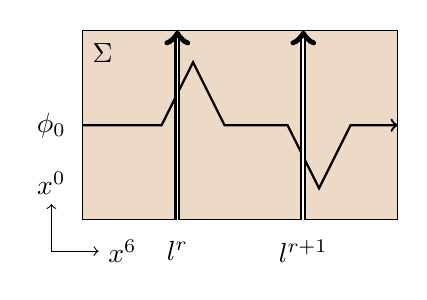
\begin{tikzpicture}[scale=0.4, baseline=(x.base)]
      \node (x) at (0,0) {\vphantom{x}};

      \draw[fill=brown!30] (0,0) rectangle (10,6);
      % \draw[step=0.5,gray,very thin] (0,0) grid (10,6);

      \draw[thick, ->] (0,3) -- (2.5,3) -- (3.5,5) -- (4.5,3) --
      (6.5,3) -- (7.5,1) -- (8.5,3) -- (10,3);

      \draw[thick, double, ->] (3,0) -- +(90:6);
      \draw[thick, double, ->] (7,0) -- +(90:6);

      \node[right] at (0,5.3) {$\Sigma$};

      \draw[->] (-1,-1) -- +(90:1.5) node[above] {$x^0$};
      \draw[->] (-1,-1) -- +(0:1.5) node[right] {$x^6$};

      \node at (-1,3) {$\phi_0$};
      \node at (3,-1) {$l^r$};
      \node at (7,-1) {$l^{r+1}$};
    \end{tikzpicture}
  }
  \qquad
  \subfloat[]{
    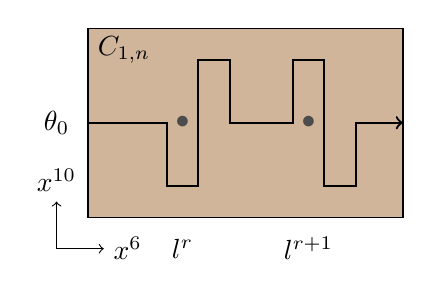
\begin{tikzpicture}[scale=0.4, baseline=(x.base)]
      \node (x) at (0,0) {\vphantom{x}};

      \draw[fill={rgb,255:red,208; green,181; blue,155}] (0,0) rectangle (10,6);
      % \draw[step=0.5,gray,very thin] (0,0) grid (10,6);

      \node[black!70] (p1) at (3,3) {$\bullet$};
      \node[black!70] (p2) at (7,3) {$\bullet$};

      \draw[thick, ->] (0,3) -- (2.5,3) -- (2.5,1) -- (3.5,1) -- (3.5,5) -- (4.5,5) -- (4.5,3) -- (6.5,3) -- (6.5,5) -- (7.5,5) -- (7.5,1) -- (8.5,1) -- (8.5,3) -- (10,3);

      \node[right] at (0,5.3) {$C_{1,n}$};

      \draw[->] (-1,-1) -- +(90:1.5) node[above] {$x^{10}$};
      \draw[->] (-1,-1) -- +(0:1.5) node[right] {$x^6$};

      \node at (-1,3) {$\theta_0$};
      \node at (3,-1) {$l^r$};
      \node at (7,-1) {$l^{r+1}$};
    \end{tikzpicture}
  }
  \caption{(a) A path in $\Sigma$ bending near solid lines.  (b) The
    corresponding path in $C_{1,n}$ detours around the punctures.}
  \label{fig:path-4dCS}
\end{figure}

The trigonometric limit $\check{R}_9 \to 0$ is equivalent to the limit
$R_{10} \to \infty$.  In this limit, $C_{1,n}$ is elongated by an
infinite factor in the $x^{10}$-direction and the dashed line is
located at $z = l^r - \sigma^r \iu\infty$ when it crosses the $r$th
solid line.  This is precisely the limit that appears in the
definitions of the fundamental L-operators~\eqref{eq:fund-L}, from
which $\CT_{\sigma,m}$ is constructed.

The D5--NS5--D3 brane system~\eqref{eq:M-D5}--\eqref{eq:M-D3} is
another interesting duality frame.  It is actually possible to
introduce an additional set of NS5-branes so that the 5-brane system
realizes a four-dimensional $\CN = 1$ supersymmetric gauge theory on
$\R^2_{12} \times_\eps S^1_3 \times \check S^1_9$.  The D3-brane
creates a surface defect in this theory.  As expected, it acts on the
partition function of the theory as an elliptic transfer
matrix~\cite{Maruyoshi:2016caf,Yagi:2017hmj}.





%%%%%%%%%%%%%%%%%%%%%%%%%%%%%%%%%%%%%%%%%%%%%%%%%%%%%%%%%



\bibliographystyle{Common/utphys}
%\nocite{*}
\bibliography{Common/Ref}



\end{document}